\documentclass[twoside]{book}

% Packages required by doxygen
\usepackage{fixltx2e}
\usepackage{calc}
\usepackage{doxygen}
\usepackage[export]{adjustbox} % also loads graphicx
\usepackage{graphicx}
\usepackage[utf8]{inputenc}
\usepackage{makeidx}
\usepackage{multicol}
\usepackage{multirow}
\PassOptionsToPackage{warn}{textcomp}
\usepackage{textcomp}
\usepackage[nointegrals]{wasysym}
\usepackage[table]{xcolor}

% Font selection
\usepackage[T1]{fontenc}
\usepackage[scaled=.90]{helvet}
\usepackage{courier}
\usepackage{amssymb}
\usepackage{sectsty}
\renewcommand{\familydefault}{\sfdefault}
\allsectionsfont{%
  \fontseries{bc}\selectfont%
  \color{darkgray}%
}
\renewcommand{\DoxyLabelFont}{%
  \fontseries{bc}\selectfont%
  \color{darkgray}%
}
\newcommand{\+}{\discretionary{\mbox{\scriptsize$\hookleftarrow$}}{}{}}

% Page & text layout
\usepackage{geometry}
\geometry{%
  a4paper,%
  top=2.5cm,%
  bottom=2.5cm,%
  left=2.5cm,%
  right=2.5cm%
}
\tolerance=750
\hfuzz=15pt
\hbadness=750
\setlength{\emergencystretch}{15pt}
\setlength{\parindent}{0cm}
\setlength{\parskip}{3ex plus 2ex minus 2ex}
\makeatletter
\renewcommand{\paragraph}{%
  \@startsection{paragraph}{4}{0ex}{-1.0ex}{1.0ex}{%
    \normalfont\normalsize\bfseries\SS@parafont%
  }%
}
\renewcommand{\subparagraph}{%
  \@startsection{subparagraph}{5}{0ex}{-1.0ex}{1.0ex}{%
    \normalfont\normalsize\bfseries\SS@subparafont%
  }%
}
\makeatother

% Headers & footers
\usepackage{fancyhdr}
\pagestyle{fancyplain}
\fancyhead[LE]{\fancyplain{}{\bfseries\thepage}}
\fancyhead[CE]{\fancyplain{}{}}
\fancyhead[RE]{\fancyplain{}{\bfseries\leftmark}}
\fancyhead[LO]{\fancyplain{}{\bfseries\rightmark}}
\fancyhead[CO]{\fancyplain{}{}}
\fancyhead[RO]{\fancyplain{}{\bfseries\thepage}}
\fancyfoot[LE]{\fancyplain{}{}}
\fancyfoot[CE]{\fancyplain{}{}}
\fancyfoot[RE]{\fancyplain{}{\bfseries\scriptsize Generated by Doxygen }}
\fancyfoot[LO]{\fancyplain{}{\bfseries\scriptsize Generated by Doxygen }}
\fancyfoot[CO]{\fancyplain{}{}}
\fancyfoot[RO]{\fancyplain{}{}}
\renewcommand{\footrulewidth}{0.4pt}
\renewcommand{\chaptermark}[1]{%
  \markboth{#1}{}%
}
\renewcommand{\sectionmark}[1]{%
  \markright{\thesection\ #1}%
}

% Indices & bibliography
\usepackage{natbib}
\usepackage[titles]{tocloft}
\setcounter{tocdepth}{3}
\setcounter{secnumdepth}{5}
\makeindex

% Hyperlinks (required, but should be loaded last)
\usepackage{ifpdf}
\ifpdf
  \usepackage[pdftex,pagebackref=true]{hyperref}
\else
  \usepackage[ps2pdf,pagebackref=true]{hyperref}
\fi
\hypersetup{%
  colorlinks=true,%
  linkcolor=blue,%
  citecolor=blue,%
  unicode%
}

% Custom commands
\newcommand{\clearemptydoublepage}{%
  \newpage{\pagestyle{empty}\cleardoublepage}%
}

\usepackage{caption}
\captionsetup{labelsep=space,justification=centering,font={bf},singlelinecheck=off,skip=4pt,position=top}

%===== C O N T E N T S =====

\begin{document}

% Titlepage & ToC
\hypersetup{pageanchor=false,
             bookmarksnumbered=true,
             pdfencoding=unicode
            }
\pagenumbering{alph}
\begin{titlepage}
\vspace*{7cm}
\begin{center}%
{\Large P\+R\+I\+S\+M\+\_\+\+S\+IM }\\
\vspace*{1cm}
{\large Generated by Doxygen 1.8.12}\\
\end{center}
\end{titlepage}
\clearemptydoublepage
\pagenumbering{roman}
\tableofcontents
\clearemptydoublepage
\pagenumbering{arabic}
\hypersetup{pageanchor=true}

%--- Begin generated contents ---
\chapter{Hierarchical Index}
\section{Class Hierarchy}
This inheritance list is sorted roughly, but not completely, alphabetically\+:\begin{DoxyCompactList}
\item \contentsline{section}{Angles}{\pageref{struct_angles}}{}
\item G4\+U\+Imessenger\begin{DoxyCompactList}
\item \contentsline{section}{Detector\+Construction\+Messenger}{\pageref{class_detector_construction_messenger}}{}
\item \contentsline{section}{Primary\+Generator\+Action\+Messenger}{\pageref{class_primary_generator_action_messenger}}{}
\item \contentsline{section}{Stacking\+Action\+Messenger}{\pageref{class_stacking_action_messenger}}{}
\end{DoxyCompactList}
\item G4\+User\+Event\+Action\begin{DoxyCompactList}
\item \contentsline{section}{Event\+Action}{\pageref{class_event_action}}{}
\end{DoxyCompactList}
\item G4\+User\+Run\+Action\begin{DoxyCompactList}
\item \contentsline{section}{Run\+Action}{\pageref{class_run_action}}{}
\end{DoxyCompactList}
\item G4\+User\+Stacking\+Action\begin{DoxyCompactList}
\item \contentsline{section}{Stacking\+Action}{\pageref{class_stacking_action}}{}
\end{DoxyCompactList}
\item G4\+User\+Stepping\+Action\begin{DoxyCompactList}
\item \contentsline{section}{Stepping\+Action}{\pageref{class_stepping_action}}{}
\end{DoxyCompactList}
\item G4\+V\+Hit\begin{DoxyCompactList}
\item \contentsline{section}{Hit}{\pageref{class_hit}}{}
\end{DoxyCompactList}
\item G4\+V\+Sensitive\+Detector\begin{DoxyCompactList}
\item \contentsline{section}{Sensitive\+Detector}{\pageref{class_sensitive_detector}}{}
\end{DoxyCompactList}
\item G4\+V\+User\+Action\+Initialization\begin{DoxyCompactList}
\item \contentsline{section}{Action\+Initialization}{\pageref{class_action_initialization}}{}
\end{DoxyCompactList}
\item G4\+V\+User\+Detector\+Construction\begin{DoxyCompactList}
\item \contentsline{section}{Detector\+Construction}{\pageref{class_detector_construction}}{}
\end{DoxyCompactList}
\item G4\+V\+User\+Physics\+List\begin{DoxyCompactList}
\item \contentsline{section}{Physics\+List}{\pageref{class_physics_list}}{}
\end{DoxyCompactList}
\item G4\+V\+User\+Primary\+Generator\+Action\begin{DoxyCompactList}
\item \contentsline{section}{Primary\+Generator\+Action}{\pageref{class_primary_generator_action}}{}
\end{DoxyCompactList}
\item \contentsline{section}{Source\+Info}{\pageref{class_source_info}}{}
\end{DoxyCompactList}

\chapter{Class Index}
\section{Class List}
Here are the classes, structs, unions and interfaces with brief descriptions\+:\begin{DoxyCompactList}
\item\contentsline{section}{\hyperlink{class_action_initialization}{Action\+Initialization} }{\pageref{class_action_initialization}}{}
\item\contentsline{section}{\hyperlink{struct_angles}{Angles} }{\pageref{struct_angles}}{}
\item\contentsline{section}{\hyperlink{class_detector_construction}{Detector\+Construction} }{\pageref{class_detector_construction}}{}
\item\contentsline{section}{\hyperlink{class_detector_construction_messenger}{Detector\+Construction\+Messenger} }{\pageref{class_detector_construction_messenger}}{}
\item\contentsline{section}{\hyperlink{class_event_action}{Event\+Action} }{\pageref{class_event_action}}{}
\item\contentsline{section}{\hyperlink{class_hit}{Hit} }{\pageref{class_hit}}{}
\item\contentsline{section}{\hyperlink{class_physics_list}{Physics\+List} }{\pageref{class_physics_list}}{}
\item\contentsline{section}{\hyperlink{class_primary_generator_action}{Primary\+Generator\+Action} }{\pageref{class_primary_generator_action}}{}
\item\contentsline{section}{\hyperlink{class_primary_generator_action_messenger}{Primary\+Generator\+Action\+Messenger} }{\pageref{class_primary_generator_action_messenger}}{}
\item\contentsline{section}{\hyperlink{class_run_action}{Run\+Action} }{\pageref{class_run_action}}{}
\item\contentsline{section}{\hyperlink{class_sensitive_detector}{Sensitive\+Detector} }{\pageref{class_sensitive_detector}}{}
\item\contentsline{section}{\hyperlink{class_source_info}{Source\+Info} }{\pageref{class_source_info}}{}
\item\contentsline{section}{\hyperlink{class_stacking_action}{Stacking\+Action} }{\pageref{class_stacking_action}}{}
\item\contentsline{section}{\hyperlink{class_stacking_action_messenger}{Stacking\+Action\+Messenger} }{\pageref{class_stacking_action_messenger}}{}
\item\contentsline{section}{\hyperlink{class_stepping_action}{Stepping\+Action} }{\pageref{class_stepping_action}}{}
\end{DoxyCompactList}

\chapter{Class Documentation}
\hypertarget{class_action_initialization}{}\section{Action\+Initialization Class Reference}
\label{class_action_initialization}\index{Action\+Initialization@{Action\+Initialization}}
Inheritance diagram for Action\+Initialization\+:\begin{figure}[H]
\begin{center}
\leavevmode
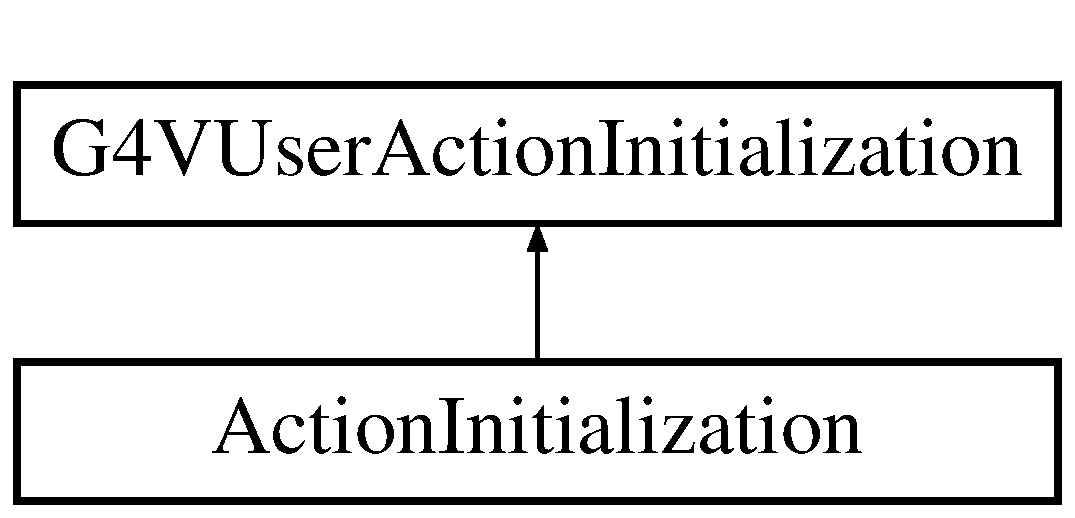
\includegraphics[height=2.000000cm]{class_action_initialization}
\end{center}
\end{figure}
\subsection*{Public Member Functions}
\begin{DoxyCompactItemize}
\item 
\hypertarget{class_action_initialization_a48c24b5a340ef3e8a69f44f9b6bf02be}{}\label{class_action_initialization_a48c24b5a340ef3e8a69f44f9b6bf02be} 
virtual void {\bfseries Build\+For\+Master} () const
\item 
\hypertarget{class_action_initialization_a9b8f6328b1b2e3ba39a1c230774cab66}{}\label{class_action_initialization_a9b8f6328b1b2e3ba39a1c230774cab66} 
virtual void {\bfseries Build} () const
\end{DoxyCompactItemize}


The documentation for this class was generated from the following files\+:\begin{DoxyCompactItemize}
\item 
/\+Users/\+Hellfeld/\+Documents/\+School/\+U\+C\+B/\+Research/\+P\+R\+I\+S\+M/\+Simulations/\+P\+R\+I\+S\+M\+\_\+\+Sim/\+P\+R\+I\+S\+M\+\_\+\+Sim/include/Action\+Initialization.\+hh\item 
/\+Users/\+Hellfeld/\+Documents/\+School/\+U\+C\+B/\+Research/\+P\+R\+I\+S\+M/\+Simulations/\+P\+R\+I\+S\+M\+\_\+\+Sim/\+P\+R\+I\+S\+M\+\_\+\+Sim/src/Action\+Initialization.\+cc\end{DoxyCompactItemize}

\hypertarget{struct_angles}{}\section{Angles Struct Reference}
\label{struct_angles}\index{Angles@{Angles}}
\subsection*{Public Attributes}
\begin{DoxyCompactItemize}
\item 
\hypertarget{struct_angles_aa462c67b8885678826e948ac0c4df7c9}{}\label{struct_angles_aa462c67b8885678826e948ac0c4df7c9} 
G4double {\bfseries theta}
\item 
\hypertarget{struct_angles_acb157a5857a39850063b0e6dfc03c509}{}\label{struct_angles_acb157a5857a39850063b0e6dfc03c509} 
G4double {\bfseries phi}
\end{DoxyCompactItemize}


The documentation for this struct was generated from the following file\+:\begin{DoxyCompactItemize}
\item 
/\+Users/\+Hellfeld/\+Documents/\+School/\+U\+C\+B/\+Research/\+P\+R\+I\+S\+M/\+Simulations/\+P\+R\+I\+S\+M\+\_\+\+Sim/\+P\+R\+I\+S\+M\+\_\+\+Sim/include/Primary\+Generator\+Action.\+hh\end{DoxyCompactItemize}

\hypertarget{class_detector_construction}{}\section{Detector\+Construction Class Reference}
\label{class_detector_construction}\index{Detector\+Construction@{Detector\+Construction}}
Inheritance diagram for Detector\+Construction\+:\begin{figure}[H]
\begin{center}
\leavevmode
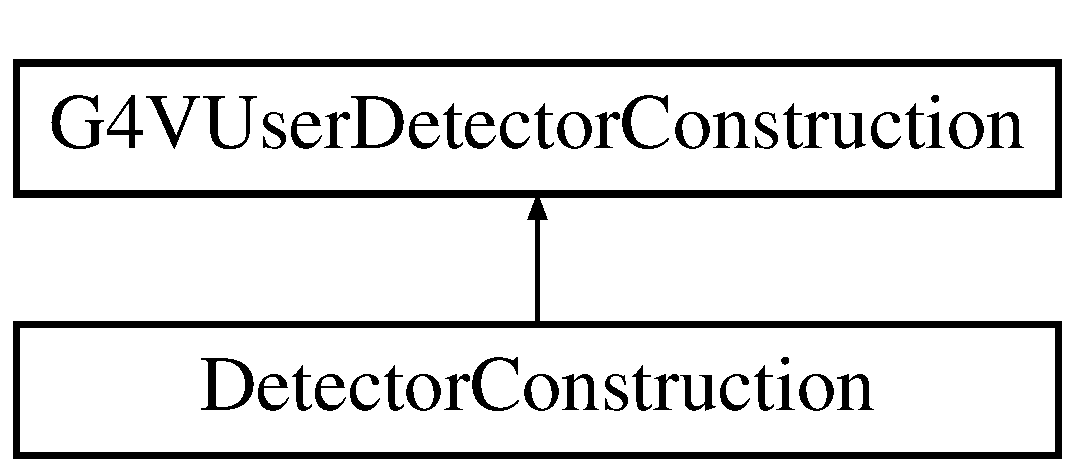
\includegraphics[height=2.000000cm]{class_detector_construction}
\end{center}
\end{figure}
\subsection*{Public Member Functions}
\begin{DoxyCompactItemize}
\item 
\hypertarget{class_detector_construction_a662c618480b345a747f014b845d5ffdf}{}\label{class_detector_construction_a662c618480b345a747f014b845d5ffdf} 
G4\+V\+Physical\+Volume $\ast$ {\bfseries Construct} ()
\item 
\hypertarget{class_detector_construction_a95c3a4dc131ffdf4cc575b3969f32761}{}\label{class_detector_construction_a95c3a4dc131ffdf4cc575b3969f32761} 
const G4double \& {\bfseries Get\+World\+Dimensions} () const
\item 
\hypertarget{class_detector_construction_a6a1e35c537ff4b9008c179e8fb13e376}{}\label{class_detector_construction_a6a1e35c537ff4b9008c179e8fb13e376} 
const G4\+Three\+Vector \& {\bfseries Get\+Target\+Position} () const
\item 
\hypertarget{class_detector_construction_a507c12633a16921409ad3435b2eca02d}{}\label{class_detector_construction_a507c12633a16921409ad3435b2eca02d} 
const G4\+Three\+Vector \& {\bfseries Get\+Target\+Dimension} () const
\item 
\hypertarget{class_detector_construction_aa88426683f97c31c8053004bd6952751}{}\label{class_detector_construction_aa88426683f97c31c8053004bd6952751} 
virtual void {\bfseries Construct\+S\+Dand\+Field} ()
\item 
\hypertarget{class_detector_construction_a13b7d1b5ce00cc50f810d507c3e2fb75}{}\label{class_detector_construction_a13b7d1b5ce00cc50f810d507c3e2fb75} 
vector$<$ G4int $>$ {\bfseries Get\+Random\+Mask} ()
\item 
\hypertarget{class_detector_construction_a6ec732600c5b5f387a447fc1377d9fd8}{}\label{class_detector_construction_a6ec732600c5b5f387a447fc1377d9fd8} 
vector$<$ G4int $>$ {\bfseries Get\+Full\+Mask} ()
\item 
\hypertarget{class_detector_construction_ac719dce27c524cc9b99e90b5b3296eca}{}\label{class_detector_construction_ac719dce27c524cc9b99e90b5b3296eca} 
void {\bfseries Set\+Mask} (vector$<$ G4int $>$)
\item 
\hypertarget{class_detector_construction_a7a3259a049a631293a36d2ee143ae6ff}{}\label{class_detector_construction_a7a3259a049a631293a36d2ee143ae6ff} 
G4\+String {\bfseries Bin\+To\+Hex} (vector$<$ G4int $>$)
\item 
\hypertarget{class_detector_construction_a47c0235d84d71a08ad014a794d4e8899}{}\label{class_detector_construction_a47c0235d84d71a08ad014a794d4e8899} 
vector$<$ G4int $>$ {\bfseries Hex\+To\+Bin} (G4\+String)
\item 
\hypertarget{class_detector_construction_a2742ef0ae83433992902a56693f2c6e5}{}\label{class_detector_construction_a2742ef0ae83433992902a56693f2c6e5} 
void {\bfseries Update\+Geometry} ()
\item 
\hypertarget{class_detector_construction_aad284f21239ea4e1f180f5c09e464bc4}{}\label{class_detector_construction_aad284f21239ea4e1f180f5c09e464bc4} 
void {\bfseries Set\+Det\+Dim} (G4\+Three\+Vector)
\item 
\hypertarget{class_detector_construction_a863b154ff7ba8dbfc86117a62ac53b93}{}\label{class_detector_construction_a863b154ff7ba8dbfc86117a62ac53b93} 
void {\bfseries Check\+Overlaps\+On} ()
\item 
\hypertarget{class_detector_construction_a3d77b1fc69db8fad1d4ff8f42409eb29}{}\label{class_detector_construction_a3d77b1fc69db8fad1d4ff8f42409eb29} 
vector$<$ G4\+Three\+Vector $>$ {\bfseries Get\+Det\+Centers} ()
\item 
\hypertarget{class_detector_construction_a0587765cb3f7e035fd355bac97d11141}{}\label{class_detector_construction_a0587765cb3f7e035fd355bac97d11141} 
vector$<$ G4\+Rotation\+Matrix $>$ {\bfseries Get\+Rotation\+Mat} ()
\item 
\hypertarget{class_detector_construction_a3dec0f5c03b83ef31bc78890a60cb1b9}{}\label{class_detector_construction_a3dec0f5c03b83ef31bc78890a60cb1b9} 
void {\bfseries Set\+Det\+Indexing} (G4\+String di)
\item 
\hypertarget{class_detector_construction_a0aeae93f2119338df2e3dd88508afb82}{}\label{class_detector_construction_a0aeae93f2119338df2e3dd88508afb82} 
G4\+String {\bfseries Get\+Det\+Indexing} ()
\end{DoxyCompactItemize}
\subsection*{Static Public Member Functions}
\begin{DoxyCompactItemize}
\item 
\hypertarget{class_detector_construction_ab85e322ba1122fe6f60a58448a36ad7a}{}\label{class_detector_construction_ab85e322ba1122fe6f60a58448a36ad7a} 
static \hyperlink{class_detector_construction}{Detector\+Construction} $\ast$ {\bfseries Instance} ()
\end{DoxyCompactItemize}
\subsection*{Public Attributes}
\begin{DoxyCompactItemize}
\item 
\hypertarget{class_detector_construction_a28fb420a8023ce56fd479794087fc778}{}\label{class_detector_construction_a28fb420a8023ce56fd479794087fc778} 
\hyperlink{class_detector_construction_messenger}{Detector\+Construction\+Messenger} $\ast$ {\bfseries detectorconstructionmessenger}
\item 
\hypertarget{class_detector_construction_a02ae227b79157d974ff0e20ab6838825}{}\label{class_detector_construction_a02ae227b79157d974ff0e20ab6838825} 
vector$<$ G4\+Three\+Vector $>$ {\bfseries centers}
\item 
\hypertarget{class_detector_construction_a61939a679302d23204e8293c1e55a464}{}\label{class_detector_construction_a61939a679302d23204e8293c1e55a464} 
vector$<$ G4\+Rotation\+Matrix $>$ {\bfseries rotationmat}
\item 
\hypertarget{class_detector_construction_a5c54b134335b03a63974a411cec5441a}{}\label{class_detector_construction_a5c54b134335b03a63974a411cec5441a} 
G4\+String {\bfseries detindexing}
\end{DoxyCompactItemize}
\subsection*{Protected Member Functions}
\begin{DoxyCompactItemize}
\item 
\hypertarget{class_detector_construction_ab07aa7cce0b67683a2278ffe983f1704}{}\label{class_detector_construction_ab07aa7cce0b67683a2278ffe983f1704} 
virtual G4\+V\+Physical\+Volume $\ast$ {\bfseries Construct\+World} ()
\item 
\hypertarget{class_detector_construction_a2d88bc1a46d1d816ba63c0b488964ff4}{}\label{class_detector_construction_a2d88bc1a46d1d816ba63c0b488964ff4} 
virtual void {\bfseries Construct\+Materials} ()
\end{DoxyCompactItemize}
\subsection*{Protected Attributes}
\begin{DoxyCompactItemize}
\item 
\hypertarget{class_detector_construction_a1a10548a1daef32cd566a3fdcba07cd7}{}\label{class_detector_construction_a1a10548a1daef32cd566a3fdcba07cd7} 
G4\+V\+Physical\+Volume $\ast$ {\bfseries world\+Phys}
\item 
\hypertarget{class_detector_construction_a5dcb068f4f80d532062eb7ec11a49b4a}{}\label{class_detector_construction_a5dcb068f4f80d532062eb7ec11a49b4a} 
G4\+Material $\ast$ {\bfseries mworld}
\item 
\hypertarget{class_detector_construction_ae8fdb511783bd31d3b430ba2a6bf39d8}{}\label{class_detector_construction_ae8fdb511783bd31d3b430ba2a6bf39d8} 
G4\+Material $\ast$ {\bfseries mdetector}
\item 
\hypertarget{class_detector_construction_a6a90b0ff0da8c387b6ee3d0c324fb4ae}{}\label{class_detector_construction_a6a90b0ff0da8c387b6ee3d0c324fb4ae} 
G4double {\bfseries world\+\_\+dim}
\item 
\hypertarget{class_detector_construction_a411b4a80cdd1233eca1b263dc9964d1a}{}\label{class_detector_construction_a411b4a80cdd1233eca1b263dc9964d1a} 
G4\+Three\+Vector {\bfseries detector\+\_\+dim}
\item 
\hypertarget{class_detector_construction_ad24de8ecffb0f690f28918f8c141161f}{}\label{class_detector_construction_ad24de8ecffb0f690f28918f8c141161f} 
G4\+Three\+Vector {\bfseries detector\+\_\+pos}
\item 
\hypertarget{class_detector_construction_a6402314fffad38b15d589778ef814dff}{}\label{class_detector_construction_a6402314fffad38b15d589778ef814dff} 
G4\+Rotation\+Matrix {\bfseries detector\+\_\+rot}
\item 
\hypertarget{class_detector_construction_ac91629e4e7bfb5e3ecd396dd556799c1}{}\label{class_detector_construction_ac91629e4e7bfb5e3ecd396dd556799c1} 
bool {\bfseries \+\_\+checkoverlaps}
\end{DoxyCompactItemize}


The documentation for this class was generated from the following files\+:\begin{DoxyCompactItemize}
\item 
/\+Users/\+Hellfeld/\+Documents/\+School/\+U\+C\+B/\+Research/\+P\+R\+I\+S\+M/\+Simulations/\+P\+R\+I\+S\+M\+\_\+\+Sim/\+P\+R\+I\+S\+M\+\_\+\+Sim/include/Detector\+Construction.\+hh\item 
/\+Users/\+Hellfeld/\+Documents/\+School/\+U\+C\+B/\+Research/\+P\+R\+I\+S\+M/\+Simulations/\+P\+R\+I\+S\+M\+\_\+\+Sim/\+P\+R\+I\+S\+M\+\_\+\+Sim/src/Detector\+Construction.\+cc\end{DoxyCompactItemize}

\hypertarget{class_detector_construction_messenger}{}\section{Detector\+Construction\+Messenger Class Reference}
\label{class_detector_construction_messenger}\index{Detector\+Construction\+Messenger@{Detector\+Construction\+Messenger}}
Inheritance diagram for Detector\+Construction\+Messenger\+:\begin{figure}[H]
\begin{center}
\leavevmode
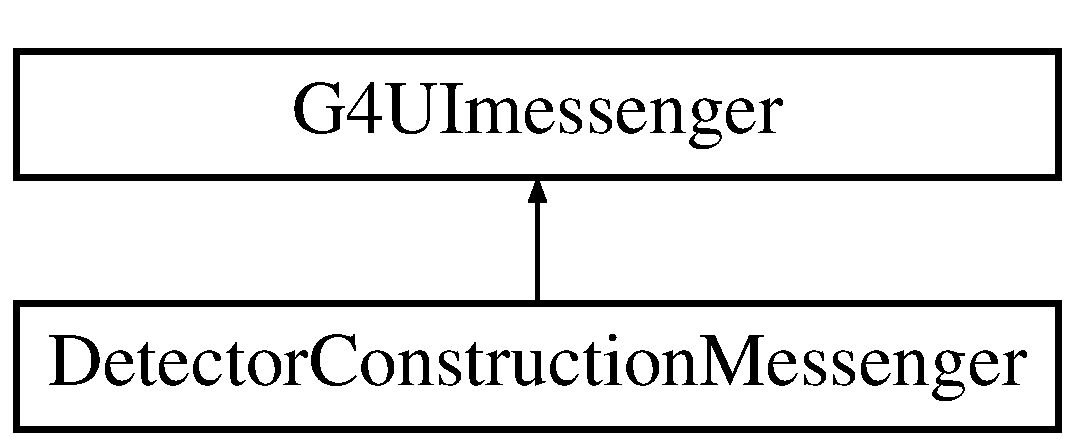
\includegraphics[height=2.000000cm]{class_detector_construction_messenger}
\end{center}
\end{figure}
\subsection*{Public Member Functions}
\begin{DoxyCompactItemize}
\item 
\hypertarget{class_detector_construction_messenger_ac67c5bc42cefea15e67863b59688b4fd}{}\label{class_detector_construction_messenger_ac67c5bc42cefea15e67863b59688b4fd} 
{\bfseries Detector\+Construction\+Messenger} (\hyperlink{class_detector_construction}{Detector\+Construction} $\ast$detector)
\item 
\hypertarget{class_detector_construction_messenger_aeff6b7186961b0212b82621412d95058}{}\label{class_detector_construction_messenger_aeff6b7186961b0212b82621412d95058} 
void {\bfseries Set\+New\+Value} (G4\+U\+Icommand $\ast$command, G4\+String new\+Value)
\end{DoxyCompactItemize}


The documentation for this class was generated from the following files\+:\begin{DoxyCompactItemize}
\item 
/\+Users/\+Hellfeld/\+Documents/\+School/\+U\+C\+B/\+Research/\+P\+R\+I\+S\+M/\+Simulations/\+P\+R\+I\+S\+M\+\_\+\+Sim/\+P\+R\+I\+S\+M\+\_\+\+Sim/include/Detector\+Construction\+Messenger.\+hh\item 
/\+Users/\+Hellfeld/\+Documents/\+School/\+U\+C\+B/\+Research/\+P\+R\+I\+S\+M/\+Simulations/\+P\+R\+I\+S\+M\+\_\+\+Sim/\+P\+R\+I\+S\+M\+\_\+\+Sim/src/Detector\+Construction\+Messenger.\+cc\end{DoxyCompactItemize}

\hypertarget{class_event_action}{}\section{Event\+Action Class Reference}
\label{class_event_action}\index{Event\+Action@{Event\+Action}}
Inheritance diagram for Event\+Action\+:\begin{figure}[H]
\begin{center}
\leavevmode
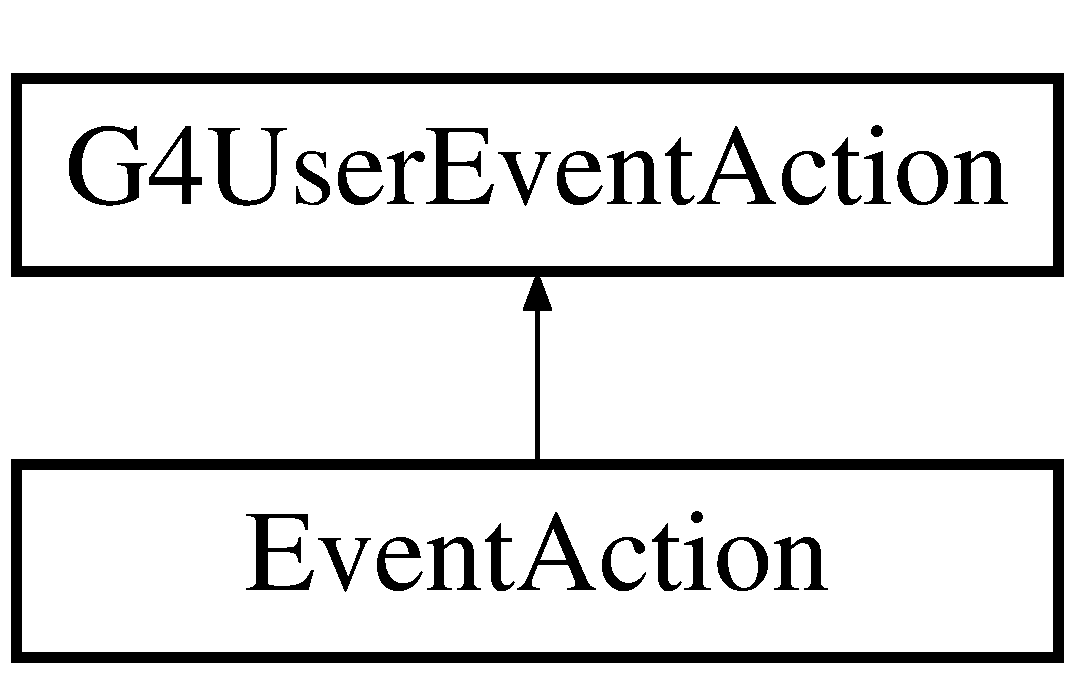
\includegraphics[height=2.000000cm]{class_event_action}
\end{center}
\end{figure}
\subsection*{Public Member Functions}
\begin{DoxyCompactItemize}
\item 
\hypertarget{class_event_action_a367abec1f640a4354f9b69e2e36e015d}{}\label{class_event_action_a367abec1f640a4354f9b69e2e36e015d} 
void {\bfseries Begin\+Of\+Event\+Action} (const G4\+Event $\ast$)
\item 
\hypertarget{class_event_action_acbb14da7b112e47ec22a253d4aa7dd4f}{}\label{class_event_action_acbb14da7b112e47ec22a253d4aa7dd4f} 
void {\bfseries End\+Of\+Event\+Action} (const G4\+Event $\ast$)
\item 
\hypertarget{class_event_action_a3d7dc3c32f0129da5d033e5bffb8a3b2}{}\label{class_event_action_a3d7dc3c32f0129da5d033e5bffb8a3b2} 
void {\bfseries Fill\+Tuples} (const G4\+Event $\ast$)
\end{DoxyCompactItemize}
\subsection*{Static Public Member Functions}
\begin{DoxyCompactItemize}
\item 
\hypertarget{class_event_action_ad3e01c4c2a8e586370bda7797fcb2e38}{}\label{class_event_action_ad3e01c4c2a8e586370bda7797fcb2e38} 
static \hyperlink{class_event_action}{Event\+Action} $\ast$ {\bfseries Instance} ()
\end{DoxyCompactItemize}


The documentation for this class was generated from the following files\+:\begin{DoxyCompactItemize}
\item 
/\+Users/\+Hellfeld/\+Documents/\+School/\+U\+C\+B/\+Research/\+P\+R\+I\+S\+M/\+Simulations/\+P\+R\+I\+S\+M\+\_\+\+Sim/\+P\+R\+I\+S\+M\+\_\+\+Sim/include/Event\+Action.\+hh\item 
/\+Users/\+Hellfeld/\+Documents/\+School/\+U\+C\+B/\+Research/\+P\+R\+I\+S\+M/\+Simulations/\+P\+R\+I\+S\+M\+\_\+\+Sim/\+P\+R\+I\+S\+M\+\_\+\+Sim/src/Event\+Action.\+cc\end{DoxyCompactItemize}

\hypertarget{class_hit}{}\section{Hit Class Reference}
\label{class_hit}\index{Hit@{Hit}}
Inheritance diagram for Hit\+:\begin{figure}[H]
\begin{center}
\leavevmode
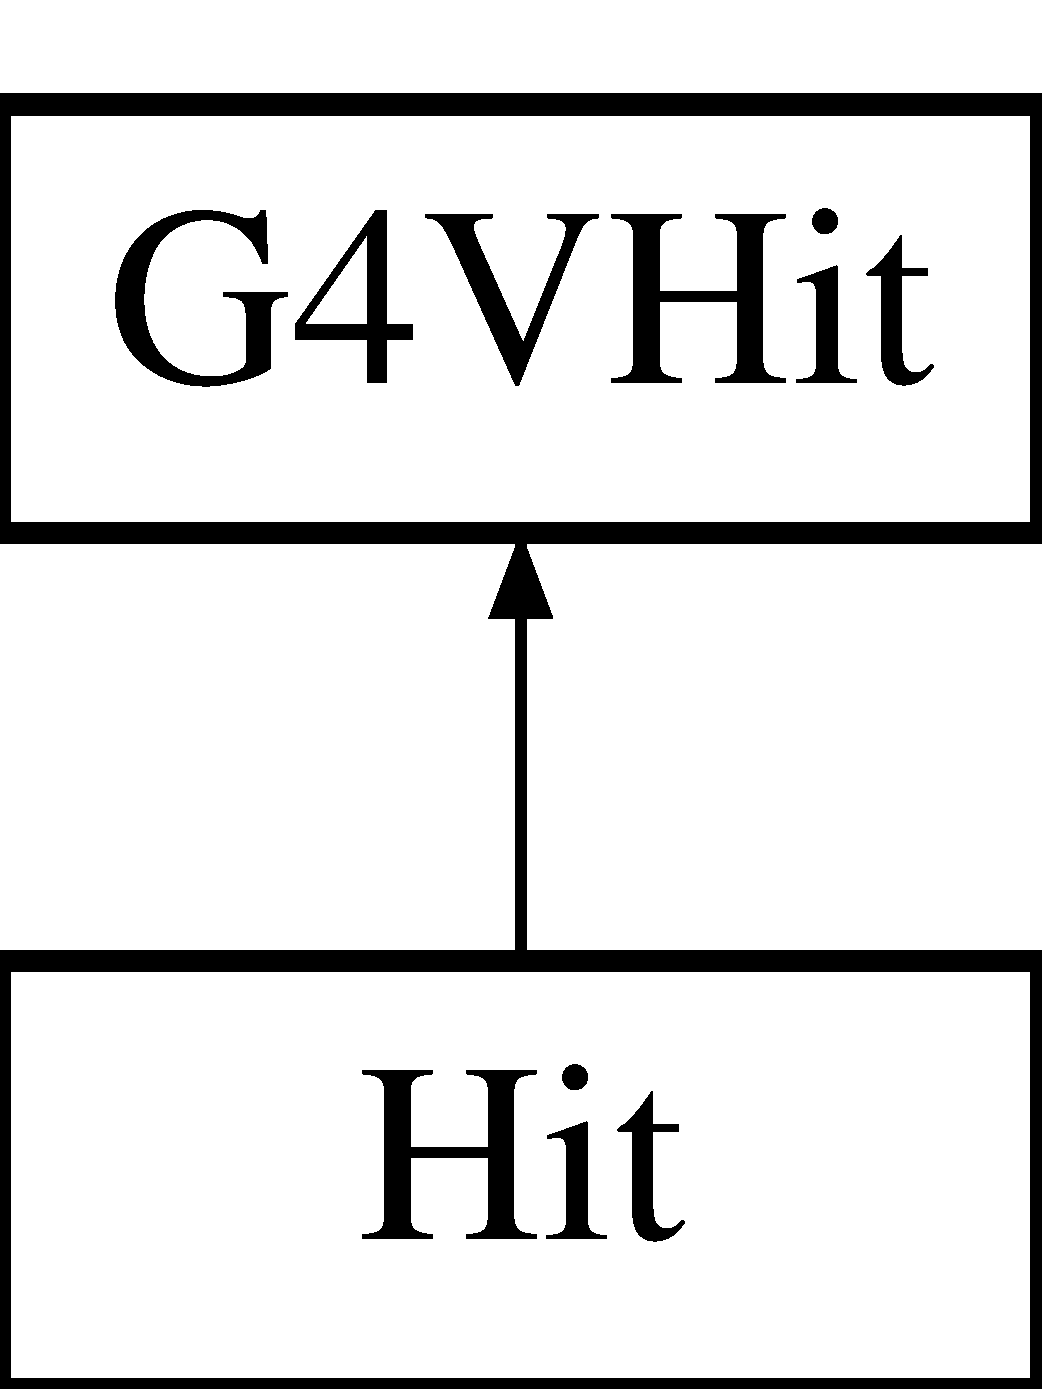
\includegraphics[height=2.000000cm]{class_hit}
\end{center}
\end{figure}
\subsection*{Public Member Functions}
\begin{DoxyCompactItemize}
\item 
\hypertarget{class_hit_aba76ed69da9702babd48e6d6fd89ddbd}{}\label{class_hit_aba76ed69da9702babd48e6d6fd89ddbd} 
{\bfseries Hit} (const \hyperlink{class_hit}{Hit} \&)
\item 
\hypertarget{class_hit_aac29fccde18f50a81d0c977a0ae8e5df}{}\label{class_hit_aac29fccde18f50a81d0c977a0ae8e5df} 
const \hyperlink{class_hit}{Hit} \& {\bfseries operator=} (const \hyperlink{class_hit}{Hit} \&)
\item 
\hypertarget{class_hit_a8176a2813547e92ace0f64e5fe428784}{}\label{class_hit_a8176a2813547e92ace0f64e5fe428784} 
G4int {\bfseries operator==} (const \hyperlink{class_hit}{Hit} \&) const
\item 
\hypertarget{class_hit_ade61deada1dde7aab01825ce3d4426fb}{}\label{class_hit_ade61deada1dde7aab01825ce3d4426fb} 
void $\ast$ {\bfseries operator new} (size\+\_\+t)
\item 
\hypertarget{class_hit_a08a30c652e131c77702231970c0f683b}{}\label{class_hit_a08a30c652e131c77702231970c0f683b} 
void {\bfseries operator delete} (void $\ast$)
\item 
\hypertarget{class_hit_a9a89a5dfbb6cc68d2795a1a200cf3076}{}\label{class_hit_a9a89a5dfbb6cc68d2795a1a200cf3076} 
void {\bfseries Set\+Track\+ID} (G4int track)
\item 
\hypertarget{class_hit_a78bab760d1e79a09cf75d5b4a6fb1435}{}\label{class_hit_a78bab760d1e79a09cf75d5b4a6fb1435} 
void {\bfseries Set\+Energy} (G4float de)
\item 
\hypertarget{class_hit_ae97cc0247c86847955835ce3d53d90d1}{}\label{class_hit_ae97cc0247c86847955835ce3d53d90d1} 
void {\bfseries Set\+Vol} (G4int volname)
\item 
\hypertarget{class_hit_aba2fe7b6fdb377ce788d57fd0bd29431}{}\label{class_hit_aba2fe7b6fdb377ce788d57fd0bd29431} 
void {\bfseries Set\+Process} (G4int procname)
\item 
\hypertarget{class_hit_a869176ee6f75f19dbf624d181498fd61}{}\label{class_hit_a869176ee6f75f19dbf624d181498fd61} 
void {\bfseries Set\+D\+OI} (G4double doi)
\item 
\hypertarget{class_hit_a268f8c747880c070149edca1fa3b831b}{}\label{class_hit_a268f8c747880c070149edca1fa3b831b} 
void {\bfseries Set\+H\+Pindex} (G4int hpindex)
\item 
\hypertarget{class_hit_a6f4b0205d9f92e35c2eb7fc4d82f2657}{}\label{class_hit_a6f4b0205d9f92e35c2eb7fc4d82f2657} 
void {\bfseries Set\+Time} (G4float time\+\_\+)
\item 
\hypertarget{class_hit_ab37a81738e892f7dbd3815711d035042}{}\label{class_hit_ab37a81738e892f7dbd3815711d035042} 
G4int {\bfseries Get\+Track\+ID} () const
\item 
\hypertarget{class_hit_a0fa28030f4260a679d6795c2a73571b6}{}\label{class_hit_a0fa28030f4260a679d6795c2a73571b6} 
G4float {\bfseries Get\+Energy} () const
\item 
\hypertarget{class_hit_af6d0ad1eed934ac7cda959d463fab795}{}\label{class_hit_af6d0ad1eed934ac7cda959d463fab795} 
G4int {\bfseries Get\+Vol} () const
\item 
\hypertarget{class_hit_a02aa237952b9ca44bf54a49aa94dc3c5}{}\label{class_hit_a02aa237952b9ca44bf54a49aa94dc3c5} 
G4int {\bfseries Get\+Process} () const
\item 
\hypertarget{class_hit_a472b618b2f916b5baee2f13924134cc3}{}\label{class_hit_a472b618b2f916b5baee2f13924134cc3} 
G4double {\bfseries Get\+D\+OI} () const
\item 
\hypertarget{class_hit_a0d71eedbcad4e5f6d14f8dd34cf3f3d3}{}\label{class_hit_a0d71eedbcad4e5f6d14f8dd34cf3f3d3} 
G4int {\bfseries Get\+H\+Pindex} () const
\item 
\hypertarget{class_hit_ac88b29254adb3500e7c1364fd053bb25}{}\label{class_hit_ac88b29254adb3500e7c1364fd053bb25} 
G4float {\bfseries Get\+Time} () const
\end{DoxyCompactItemize}


The documentation for this class was generated from the following files\+:\begin{DoxyCompactItemize}
\item 
/\+Users/\+Hellfeld/\+Documents/\+School/\+U\+C\+B/\+Research/\+P\+R\+I\+S\+M/\+Simulations/\+P\+R\+I\+S\+M\+\_\+\+Sim/\+P\+R\+I\+S\+M\+\_\+\+Sim/include/Hit.\+hh\item 
/\+Users/\+Hellfeld/\+Documents/\+School/\+U\+C\+B/\+Research/\+P\+R\+I\+S\+M/\+Simulations/\+P\+R\+I\+S\+M\+\_\+\+Sim/\+P\+R\+I\+S\+M\+\_\+\+Sim/src/Hit.\+cc\end{DoxyCompactItemize}

\hypertarget{class_physics_list}{}\section{Physics\+List Class Reference}
\label{class_physics_list}\index{Physics\+List@{Physics\+List}}
Inheritance diagram for Physics\+List\+:\begin{figure}[H]
\begin{center}
\leavevmode
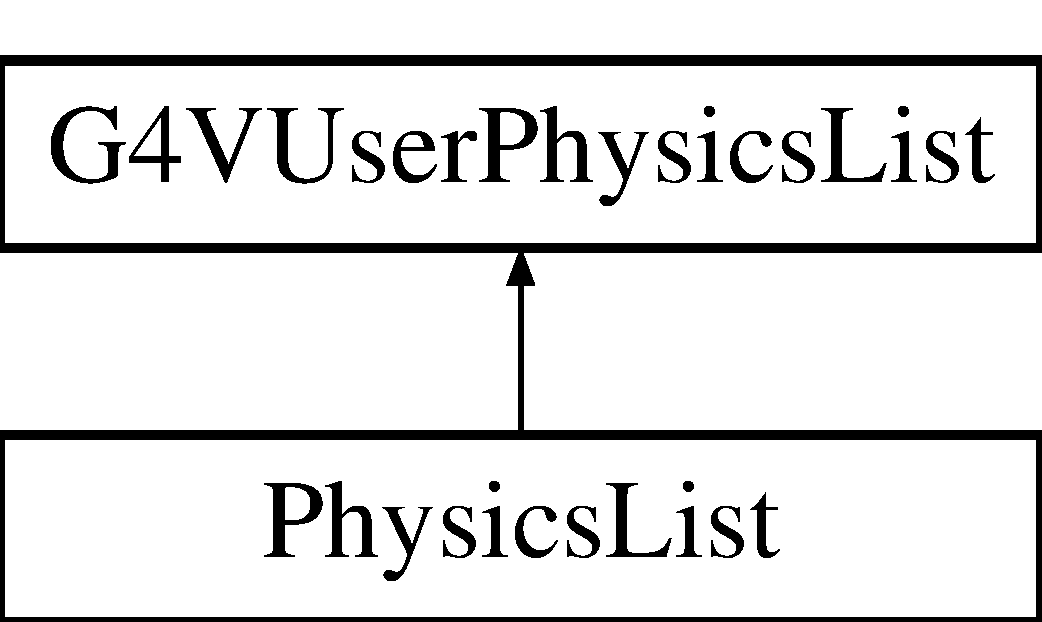
\includegraphics[height=2.000000cm]{class_physics_list}
\end{center}
\end{figure}
\subsection*{Public Member Functions}
\begin{DoxyCompactItemize}
\item 
\hypertarget{class_physics_list_af7906507122c985d2da3e61c56efe60e}{}\label{class_physics_list_af7906507122c985d2da3e61c56efe60e} 
void {\bfseries Construct\+Particle} ()
\item 
\hypertarget{class_physics_list_a9c08bc28eba2ae62104b967280901a3f}{}\label{class_physics_list_a9c08bc28eba2ae62104b967280901a3f} 
void {\bfseries Construct\+Process} ()
\item 
\hypertarget{class_physics_list_a42728fc670ddaf9404a9e023f5843c73}{}\label{class_physics_list_a42728fc670ddaf9404a9e023f5843c73} 
void {\bfseries Construct\+EM} ()
\item 
\hypertarget{class_physics_list_a0ba901b82ae30657b109930645fe8017}{}\label{class_physics_list_a0ba901b82ae30657b109930645fe8017} 
void {\bfseries Set\+Cuts} ()
\end{DoxyCompactItemize}
\subsection*{Static Public Member Functions}
\begin{DoxyCompactItemize}
\item 
\hypertarget{class_physics_list_ad9d6ed1c4ba56c39fbd5a9c29614635c}{}\label{class_physics_list_ad9d6ed1c4ba56c39fbd5a9c29614635c} 
static \hyperlink{class_physics_list}{Physics\+List} $\ast$ {\bfseries Instance} ()
\end{DoxyCompactItemize}


The documentation for this class was generated from the following files\+:\begin{DoxyCompactItemize}
\item 
/\+Users/\+Hellfeld/\+Documents/\+School/\+U\+C\+B/\+Research/\+P\+R\+I\+S\+M/\+Simulations/\+P\+R\+I\+S\+M\+\_\+\+Sim/\+P\+R\+I\+S\+M\+\_\+\+Sim/include/Physics\+List.\+hh\item 
/\+Users/\+Hellfeld/\+Documents/\+School/\+U\+C\+B/\+Research/\+P\+R\+I\+S\+M/\+Simulations/\+P\+R\+I\+S\+M\+\_\+\+Sim/\+P\+R\+I\+S\+M\+\_\+\+Sim/src/Physics\+List.\+cc\end{DoxyCompactItemize}

\hypertarget{class_primary_generator_action}{}\section{Primary\+Generator\+Action Class Reference}
\label{class_primary_generator_action}\index{Primary\+Generator\+Action@{Primary\+Generator\+Action}}
Inheritance diagram for Primary\+Generator\+Action\+:\begin{figure}[H]
\begin{center}
\leavevmode
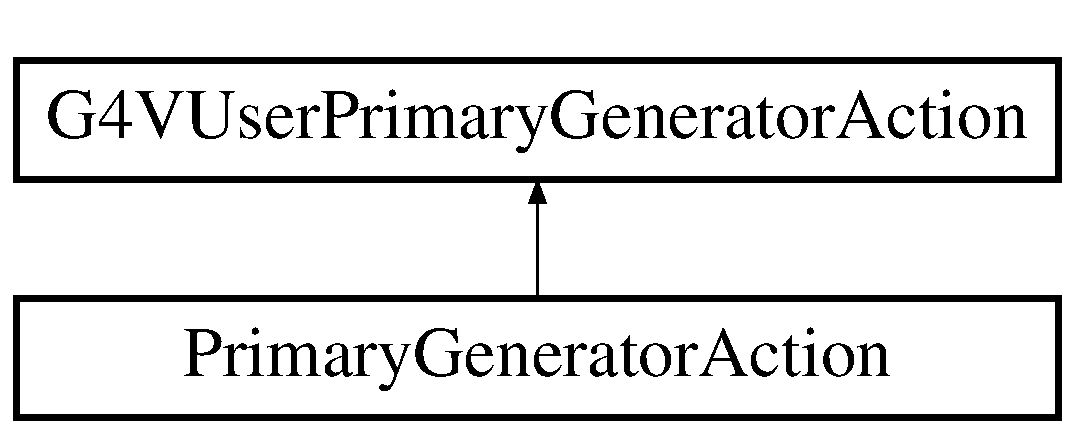
\includegraphics[height=2.000000cm]{class_primary_generator_action}
\end{center}
\end{figure}
\subsection*{Public Member Functions}
\begin{DoxyCompactItemize}
\item 
\hypertarget{class_primary_generator_action_a8c796e33304646f4d9d905dbc6f2abc5}{}\label{class_primary_generator_action_a8c796e33304646f4d9d905dbc6f2abc5} 
void {\bfseries Generate\+Primaries} (G4\+Event $\ast$)
\item 
\hypertarget{class_primary_generator_action_a46e67f9f730f414b343ee0e9a6226593}{}\label{class_primary_generator_action_a46e67f9f730f414b343ee0e9a6226593} 
void {\bfseries Set\+Theta} (G4double)
\item 
\hypertarget{class_primary_generator_action_a4615be87989e5bab795be0f3c0daada1}{}\label{class_primary_generator_action_a4615be87989e5bab795be0f3c0daada1} 
void {\bfseries Set\+Phi} (G4double)
\item 
\hypertarget{class_primary_generator_action_afb42286a618c737e0c033f2d2b2aa0c6}{}\label{class_primary_generator_action_afb42286a618c737e0c033f2d2b2aa0c6} 
\hyperlink{class_source_info}{Source\+Info} {\bfseries Far\+Field\+Source} (G4double, G4double)
\item 
\hypertarget{class_primary_generator_action_a039de9ae41c3099eedf5a18b6bb8f17a}{}\label{class_primary_generator_action_a039de9ae41c3099eedf5a18b6bb8f17a} 
\hyperlink{class_source_info}{Source\+Info} {\bfseries Near\+Field\+Source} (G4double, G4double, G4double)
\item 
\hypertarget{class_primary_generator_action_ac3e39c56ddd81eda91b7fa84a64483bd}{}\label{class_primary_generator_action_ac3e39c56ddd81eda91b7fa84a64483bd} 
\hyperlink{class_source_info}{Source\+Info} {\bfseries Far\+Field\+Ring\+Source} ()
\item 
\hypertarget{class_primary_generator_action_a57d8c467d8ca74c0de5d2f774f24ba1e}{}\label{class_primary_generator_action_a57d8c467d8ca74c0de5d2f774f24ba1e} 
void {\bfseries Set\+Far\+Field\+Source} (G4bool a)
\item 
\hypertarget{class_primary_generator_action_aba4ef4e85620251297b1ee158eaea61e}{}\label{class_primary_generator_action_aba4ef4e85620251297b1ee158eaea61e} 
G4bool {\bfseries Get\+Far\+Field\+Source} ()
\item 
\hypertarget{class_primary_generator_action_a6fb956c60f2492ffda06a632e81717f5}{}\label{class_primary_generator_action_a6fb956c60f2492ffda06a632e81717f5} 
void {\bfseries Set\+Near\+Field\+Source} (G4bool a)
\item 
\hypertarget{class_primary_generator_action_aedaba6871025ef9766ac3ee419bd3c36}{}\label{class_primary_generator_action_aedaba6871025ef9766ac3ee419bd3c36} 
G4bool {\bfseries Get\+Near\+Field\+Source} ()
\item 
\hypertarget{class_primary_generator_action_a959717f88e8e17c7dc2d3f5799bee51a}{}\label{class_primary_generator_action_a959717f88e8e17c7dc2d3f5799bee51a} 
void {\bfseries Set\+Near\+Field\+Source\+Dist} (G4double a)
\item 
\hypertarget{class_primary_generator_action_a39dae28c3904ca77a3ea0827c277692f}{}\label{class_primary_generator_action_a39dae28c3904ca77a3ea0827c277692f} 
G4double {\bfseries Get\+Near\+Field\+Source\+Dist} ()
\item 
\hypertarget{class_primary_generator_action_aa56d45fe931cdf7846379dfb33f7cd94}{}\label{class_primary_generator_action_aa56d45fe931cdf7846379dfb33f7cd94} 
void {\bfseries Set\+Far\+Field\+Ring\+Source} (G4bool a)
\item 
\hypertarget{class_primary_generator_action_af2613b6c4c0266430e8e45c95682181b}{}\label{class_primary_generator_action_af2613b6c4c0266430e8e45c95682181b} 
G4bool {\bfseries Get\+Far\+Field\+Ring\+Source} ()
\item 
\hypertarget{class_primary_generator_action_ae6d468bc4fd353e713b224ca9b8b4670}{}\label{class_primary_generator_action_ae6d468bc4fd353e713b224ca9b8b4670} 
G4int {\bfseries Get\+Acquisition\+Time} ()
\item 
\hypertarget{class_primary_generator_action_a4fee48f6be51e62a1e191e30b9330a11}{}\label{class_primary_generator_action_a4fee48f6be51e62a1e191e30b9330a11} 
void {\bfseries Set\+Acquisition\+Time} (G4int a)
\item 
\hypertarget{class_primary_generator_action_aed9c40b04be8782c7a1f609466047dba}{}\label{class_primary_generator_action_aed9c40b04be8782c7a1f609466047dba} 
G4double {\bfseries Get\+Source\+Strength} ()
\item 
\hypertarget{class_primary_generator_action_a829f96ff74f55414cb5476c2feaa1bb4}{}\label{class_primary_generator_action_a829f96ff74f55414cb5476c2feaa1bb4} 
void {\bfseries Set\+Source\+Strength} (G4double a)
\item 
\hypertarget{class_primary_generator_action_a24afde050734fff1940861d923f4dab3}{}\label{class_primary_generator_action_a24afde050734fff1940861d923f4dab3} 
G4double {\bfseries Get\+Theta} ()
\item 
\hypertarget{class_primary_generator_action_ad32d3e2540b4118dabc85bc4606bfd15}{}\label{class_primary_generator_action_ad32d3e2540b4118dabc85bc4606bfd15} 
G4double {\bfseries Get\+Phi} ()
\item 
\hypertarget{class_primary_generator_action_a99fad0c72d37e52485afd4acff7e7e5d}{}\label{class_primary_generator_action_a99fad0c72d37e52485afd4acff7e7e5d} 
void {\bfseries Set\+H\+P\+\_\+index} (G4int)
\item 
\hypertarget{class_primary_generator_action_af33801f8ff9b0335dd160dafb4b2d7a0}{}\label{class_primary_generator_action_af33801f8ff9b0335dd160dafb4b2d7a0} 
G4int {\bfseries Get\+H\+P\+\_\+index} ()
\item 
\hypertarget{class_primary_generator_action_a67721c44b11abfbcb0405e287a96b825}{}\label{class_primary_generator_action_a67721c44b11abfbcb0405e287a96b825} 
void {\bfseries Read\+In\+H\+E\+A\+L\+Pix\+Angles} (G4\+String)
\item 
\hypertarget{class_primary_generator_action_a28c6b3ac29a1793032f2dcbc5d3a899e}{}\label{class_primary_generator_action_a28c6b3ac29a1793032f2dcbc5d3a899e} 
vector$<$ struct \hyperlink{struct_angles}{Angles} $>$ {\bfseries Get\+H\+Pangles} ()
\item 
\hypertarget{class_primary_generator_action_a0d95e1e27da8ea3a526f9764288909e5}{}\label{class_primary_generator_action_a0d95e1e27da8ea3a526f9764288909e5} 
void {\bfseries Set\+H\+Pindexing} (G4\+String \+\_\+hpindexing)
\item 
\hypertarget{class_primary_generator_action_add419b7d496d524ad7ff22cf912738cf}{}\label{class_primary_generator_action_add419b7d496d524ad7ff22cf912738cf} 
G4\+String {\bfseries Get\+H\+Pindexing} ()
\item 
\hypertarget{class_primary_generator_action_a208b65bf1d407b7a151befa2add93987}{}\label{class_primary_generator_action_a208b65bf1d407b7a151befa2add93987} 
void {\bfseries Set\+H\+P\+Nside} (G4int \+\_\+hp\+Nside)
\item 
\hypertarget{class_primary_generator_action_a08d545a2fc17163e4d4a5ae80c5049a1}{}\label{class_primary_generator_action_a08d545a2fc17163e4d4a5ae80c5049a1} 
G4int {\bfseries Get\+H\+P\+Nside} ()
\end{DoxyCompactItemize}
\subsection*{Static Public Member Functions}
\begin{DoxyCompactItemize}
\item 
\hypertarget{class_primary_generator_action_a04d9a38c08290eb50d0848d44a80b089}{}\label{class_primary_generator_action_a04d9a38c08290eb50d0848d44a80b089} 
static \hyperlink{class_primary_generator_action}{Primary\+Generator\+Action} $\ast$ {\bfseries Instance} ()
\end{DoxyCompactItemize}
\subsection*{Public Attributes}
\begin{DoxyCompactItemize}
\item 
\hypertarget{class_primary_generator_action_addbbfc036b0156bb95d8e3daaae32490}{}\label{class_primary_generator_action_addbbfc036b0156bb95d8e3daaae32490} 
\hyperlink{class_primary_generator_action_messenger}{Primary\+Generator\+Action\+Messenger} $\ast$ {\bfseries primarygeneratoractionmessenger}
\item 
\hypertarget{class_primary_generator_action_a0cdcb956930b68ca7eb21000715cebb9}{}\label{class_primary_generator_action_a0cdcb956930b68ca7eb21000715cebb9} 
G4bool {\bfseries farfieldsource}
\item 
\hypertarget{class_primary_generator_action_a3f3c1be1aa74fbdb95394d326b229e87}{}\label{class_primary_generator_action_a3f3c1be1aa74fbdb95394d326b229e87} 
G4bool {\bfseries nearfieldsource}
\item 
\hypertarget{class_primary_generator_action_a6f61ce8b96e9296c10d05faf8da6c7cc}{}\label{class_primary_generator_action_a6f61ce8b96e9296c10d05faf8da6c7cc} 
G4double {\bfseries nearfieldsourcedist}
\item 
\hypertarget{class_primary_generator_action_a8bb37f211e060d53d08892ac18e1c032}{}\label{class_primary_generator_action_a8bb37f211e060d53d08892ac18e1c032} 
G4bool {\bfseries farfieldringsource}
\item 
\hypertarget{class_primary_generator_action_a856a6e25eaad9b8b6b06648bb11a7dc2}{}\label{class_primary_generator_action_a856a6e25eaad9b8b6b06648bb11a7dc2} 
G4int {\bfseries acqtime}
\item 
\hypertarget{class_primary_generator_action_ae79ffa0cb555fe839f318ed9fc522dd0}{}\label{class_primary_generator_action_ae79ffa0cb555fe839f318ed9fc522dd0} 
G4double {\bfseries srcstrength}
\item 
\hypertarget{class_primary_generator_action_a7b2a99da413dfd7fd3a45ebec3083e85}{}\label{class_primary_generator_action_a7b2a99da413dfd7fd3a45ebec3083e85} 
G4int {\bfseries H\+P\+\_\+index}
\item 
\hypertarget{class_primary_generator_action_a3f240345a5071bc7993dafdcfb68d088}{}\label{class_primary_generator_action_a3f240345a5071bc7993dafdcfb68d088} 
vector$<$ struct \hyperlink{struct_angles}{Angles} $>$ {\bfseries H\+Pangles}
\item 
\hypertarget{class_primary_generator_action_a87d3b8eab8564f086272a3f1159c76aa}{}\label{class_primary_generator_action_a87d3b8eab8564f086272a3f1159c76aa} 
G4\+String {\bfseries H\+Pindexing}
\item 
\hypertarget{class_primary_generator_action_a2cbc70d41722fa952536b7649e75eb09}{}\label{class_primary_generator_action_a2cbc70d41722fa952536b7649e75eb09} 
G4int {\bfseries H\+P\+\_\+\+Nside}
\end{DoxyCompactItemize}
\subsection*{Protected Member Functions}
\begin{DoxyCompactItemize}
\item 
\hypertarget{class_primary_generator_action_a040348143c8c552c155b620ba4ef0e84}{}\label{class_primary_generator_action_a040348143c8c552c155b620ba4ef0e84} 
G4\+Three\+Vector {\bfseries Get\+Isotropic\+Momentum\+Direction} () const
\item 
\hypertarget{class_primary_generator_action_ab80f80a97e9d9e7259157afd95a64fa3}{}\label{class_primary_generator_action_ab80f80a97e9d9e7259157afd95a64fa3} 
G4\+Three\+Vector {\bfseries Get\+Half\+Isotropic\+Momentum\+Direction} () const
\item 
\hypertarget{class_primary_generator_action_a63eb6aa5a357273cb4c61f25a3573bfe}{}\label{class_primary_generator_action_a63eb6aa5a357273cb4c61f25a3573bfe} 
G4\+Three\+Vector {\bfseries Get\+Cone\+Momentum\+Direction} (G4double) const
\item 
\hypertarget{class_primary_generator_action_afdfa3e6ae0e4d6867d4df4528ad97bca}{}\label{class_primary_generator_action_afdfa3e6ae0e4d6867d4df4528ad97bca} 
G4double {\bfseries Get\+Rand\+Theta} ()
\item 
\hypertarget{class_primary_generator_action_a67a51c7879b8db59054ea45797f58c50}{}\label{class_primary_generator_action_a67a51c7879b8db59054ea45797f58c50} 
G4double {\bfseries Get\+Rand\+Phi} ()
\end{DoxyCompactItemize}


The documentation for this class was generated from the following files\+:\begin{DoxyCompactItemize}
\item 
/\+Users/\+Hellfeld/\+Documents/\+School/\+U\+C\+B/\+Research/\+P\+R\+I\+S\+M/\+Simulations/\+P\+R\+I\+S\+M\+\_\+\+Sim/\+P\+R\+I\+S\+M\+\_\+\+Sim/include/Primary\+Generator\+Action.\+hh\item 
/\+Users/\+Hellfeld/\+Documents/\+School/\+U\+C\+B/\+Research/\+P\+R\+I\+S\+M/\+Simulations/\+P\+R\+I\+S\+M\+\_\+\+Sim/\+P\+R\+I\+S\+M\+\_\+\+Sim/src/Primary\+Generator\+Action.\+cc\end{DoxyCompactItemize}

\hypertarget{class_primary_generator_action_messenger}{}\section{Primary\+Generator\+Action\+Messenger Class Reference}
\label{class_primary_generator_action_messenger}\index{Primary\+Generator\+Action\+Messenger@{Primary\+Generator\+Action\+Messenger}}
Inheritance diagram for Primary\+Generator\+Action\+Messenger\+:\begin{figure}[H]
\begin{center}
\leavevmode
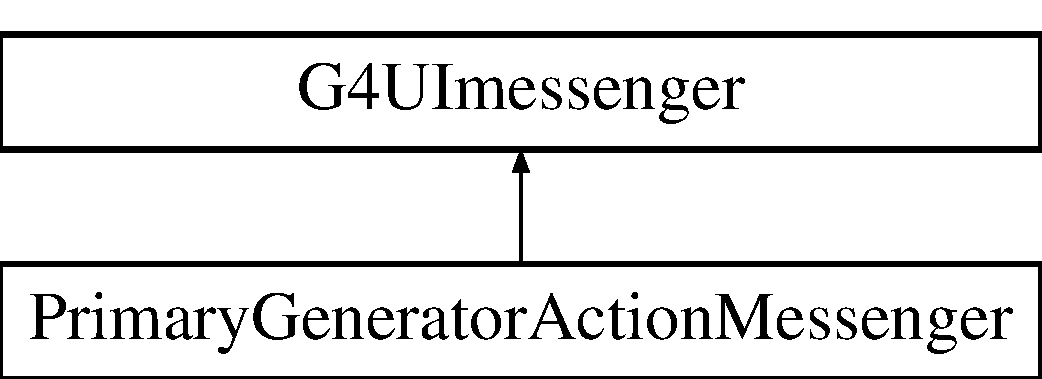
\includegraphics[height=2.000000cm]{class_primary_generator_action_messenger}
\end{center}
\end{figure}
\subsection*{Public Member Functions}
\begin{DoxyCompactItemize}
\item 
\hypertarget{class_primary_generator_action_messenger_ac5f26313e6a6232eb571ac20478ab49e}{}\label{class_primary_generator_action_messenger_ac5f26313e6a6232eb571ac20478ab49e} 
{\bfseries Primary\+Generator\+Action\+Messenger} (\hyperlink{class_primary_generator_action}{Primary\+Generator\+Action} $\ast$generator)
\item 
\hypertarget{class_primary_generator_action_messenger_a7f070eee4e7b9f8a38ea1f82147feaf4}{}\label{class_primary_generator_action_messenger_a7f070eee4e7b9f8a38ea1f82147feaf4} 
void {\bfseries Set\+New\+Value} (G4\+U\+Icommand $\ast$command, G4\+String new\+Value)
\end{DoxyCompactItemize}
\subsection*{Public Attributes}
\begin{DoxyCompactItemize}
\item 
\hypertarget{class_primary_generator_action_messenger_a7f555ea25f9f58b8d6cd706979216c02}{}\label{class_primary_generator_action_messenger_a7f555ea25f9f58b8d6cd706979216c02} 
G4\+U\+Imanager $\ast$ {\bfseries UI}
\end{DoxyCompactItemize}


The documentation for this class was generated from the following files\+:\begin{DoxyCompactItemize}
\item 
/\+Users/\+Hellfeld/\+Documents/\+School/\+U\+C\+B/\+Research/\+P\+R\+I\+S\+M/\+Simulations/\+P\+R\+I\+S\+M\+\_\+\+Sim/\+P\+R\+I\+S\+M\+\_\+\+Sim/include/Primary\+Generator\+Action\+Messenger.\+hh\item 
/\+Users/\+Hellfeld/\+Documents/\+School/\+U\+C\+B/\+Research/\+P\+R\+I\+S\+M/\+Simulations/\+P\+R\+I\+S\+M\+\_\+\+Sim/\+P\+R\+I\+S\+M\+\_\+\+Sim/src/Primary\+Generator\+Action\+Messenger.\+cc\end{DoxyCompactItemize}

\hypertarget{class_run_action}{}\section{Run\+Action Class Reference}
\label{class_run_action}\index{Run\+Action@{Run\+Action}}
Inheritance diagram for Run\+Action\+:\begin{figure}[H]
\begin{center}
\leavevmode
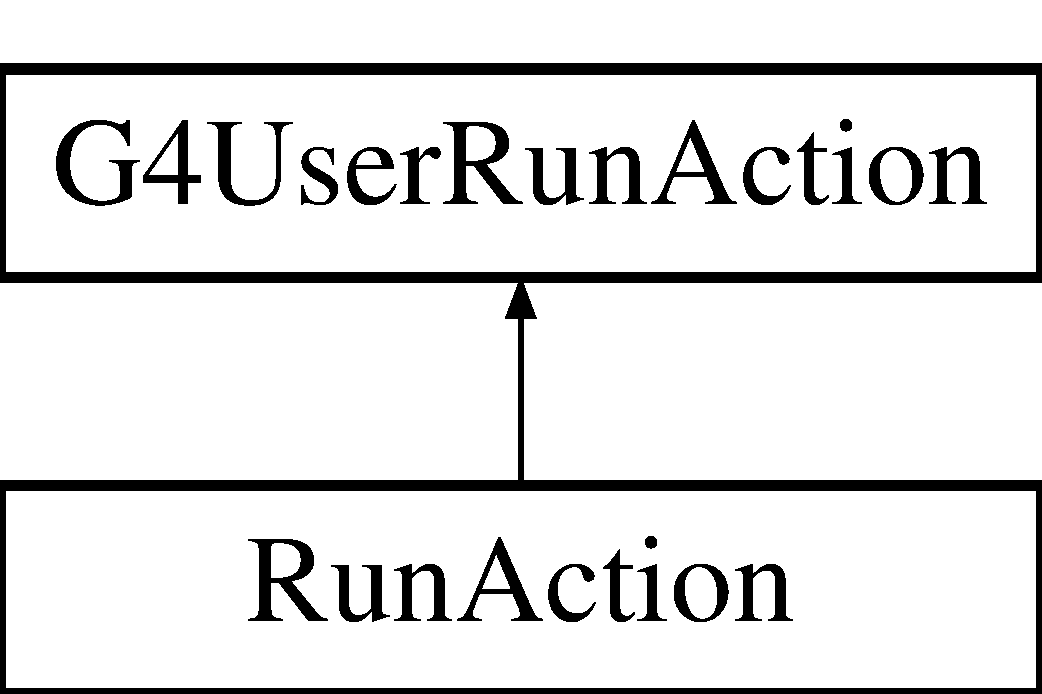
\includegraphics[height=2.000000cm]{class_run_action}
\end{center}
\end{figure}
\subsection*{Public Member Functions}
\begin{DoxyCompactItemize}
\item 
\hypertarget{class_run_action_a14b3433a6875194c4adfe1c222884f0d}{}\label{class_run_action_a14b3433a6875194c4adfe1c222884f0d} 
void {\bfseries Begin\+Of\+Run\+Action} (const G4\+Run $\ast$)
\item 
\hypertarget{class_run_action_a49e3c5db63358317c3babca100163bd9}{}\label{class_run_action_a49e3c5db63358317c3babca100163bd9} 
void {\bfseries End\+Of\+Run\+Action} (const G4\+Run $\ast$)
\item 
\hypertarget{class_run_action_a190d23b9aeea8a8712fc82c77969d0d8}{}\label{class_run_action_a190d23b9aeea8a8712fc82c77969d0d8} 
void {\bfseries Fill\+D\+O\+Ituple} (G4double)
\item 
\hypertarget{class_run_action_aee078de0e966638fc3b87fe3bc02ab55}{}\label{class_run_action_aee078de0e966638fc3b87fe3bc02ab55} 
void {\bfseries Clear\+D\+O\+Ituple} ()
\item 
\hypertarget{class_run_action_a4251d3404389fedd1fcbadafb2f3595e}{}\label{class_run_action_a4251d3404389fedd1fcbadafb2f3595e} 
vector$<$ G4double $>$ {\bfseries Get\+D\+O\+Ituple} ()
\item 
\hypertarget{class_run_action_af3f31909fcce00cb02b38384b3deaff9}{}\label{class_run_action_af3f31909fcce00cb02b38384b3deaff9} 
void {\bfseries Fill\+D\+O\+Ibintuple} (G4int)
\item 
\hypertarget{class_run_action_ad566f093dfb61cf57d7bf72cc05b4a64}{}\label{class_run_action_ad566f093dfb61cf57d7bf72cc05b4a64} 
void {\bfseries Clear\+D\+O\+Ibintuple} ()
\item 
\hypertarget{class_run_action_a83e5783caf7f1fa586d72374520c8d53}{}\label{class_run_action_a83e5783caf7f1fa586d72374520c8d53} 
vector$<$ G4int $>$ {\bfseries Get\+D\+O\+Ibintuple} ()
\item 
\hypertarget{class_run_action_a26cd79ac8520b95ccd8bdd8b7aee9ec5}{}\label{class_run_action_a26cd79ac8520b95ccd8bdd8b7aee9ec5} 
void {\bfseries Fill\+Det\+I\+Dtuple} (G4int)
\item 
\hypertarget{class_run_action_a49b4b8d75f8e4b9b4c5629c7c3c9fbc3}{}\label{class_run_action_a49b4b8d75f8e4b9b4c5629c7c3c9fbc3} 
void {\bfseries Clear\+Det\+I\+Dtuple} ()
\item 
\hypertarget{class_run_action_acc2d6a4de0722e9bcd161e403b656065}{}\label{class_run_action_acc2d6a4de0722e9bcd161e403b656065} 
vector$<$ G4int $>$ {\bfseries Get\+Det\+I\+Dtuple} ()
\item 
\hypertarget{class_run_action_a22f212b6cdca38c0b2fd7fea6f361d32}{}\label{class_run_action_a22f212b6cdca38c0b2fd7fea6f361d32} 
void {\bfseries Fill\+Evt\+Ntuple} (G4int)
\item 
\hypertarget{class_run_action_a9a26dfb552e6b5eb17ae4db9990b57cb}{}\label{class_run_action_a9a26dfb552e6b5eb17ae4db9990b57cb} 
void {\bfseries Clear\+Evt\+Ntuple} ()
\item 
\hypertarget{class_run_action_adc94bc41aca38e605436ae9ccb717bd6}{}\label{class_run_action_adc94bc41aca38e605436ae9ccb717bd6} 
vector$<$ G4int $>$ {\bfseries Get\+Evt\+Ntuple} ()
\item 
\hypertarget{class_run_action_a0bbcb3e29c7fe08c5e1407d8b135c8aa}{}\label{class_run_action_a0bbcb3e29c7fe08c5e1407d8b135c8aa} 
void {\bfseries Fill\+Hit\+Numtuple} (G4int)
\item 
\hypertarget{class_run_action_ab82fce992aaf15634afc2646b5aae72a}{}\label{class_run_action_ab82fce992aaf15634afc2646b5aae72a} 
void {\bfseries Clear\+Hit\+Numtuple} ()
\item 
\hypertarget{class_run_action_a392891d707e3a91e5bfc04e3384612ef}{}\label{class_run_action_a392891d707e3a91e5bfc04e3384612ef} 
vector$<$ G4int $>$ {\bfseries Get\+Hit\+Numtuple} ()
\item 
\hypertarget{class_run_action_aa19b8463e3dade24da0746c759191934}{}\label{class_run_action_aa19b8463e3dade24da0746c759191934} 
void {\bfseries Fill\+Track\+I\+Dtuple} (G4int)
\item 
\hypertarget{class_run_action_a182b204e689e48859627a2c32550a8ef}{}\label{class_run_action_a182b204e689e48859627a2c32550a8ef} 
void {\bfseries Clear\+Track\+I\+Dtuple} ()
\item 
\hypertarget{class_run_action_a86882b695d5a6e70401ce70ab43983f0}{}\label{class_run_action_a86882b695d5a6e70401ce70ab43983f0} 
vector$<$ G4int $>$ {\bfseries Get\+Track\+I\+Dtuple} ()
\item 
\hypertarget{class_run_action_a8bb536a43b52b9a54cfdc9b9f121a9c7}{}\label{class_run_action_a8bb536a43b52b9a54cfdc9b9f121a9c7} 
void {\bfseries Fill\+Energytuple} (G4float)
\item 
\hypertarget{class_run_action_a3b07a6e87efdafdef1fd9a2e2904408f}{}\label{class_run_action_a3b07a6e87efdafdef1fd9a2e2904408f} 
void {\bfseries Clear\+Energytuple} ()
\item 
\hypertarget{class_run_action_a83f68e07fa5cd862dd0e14941fb75ee8}{}\label{class_run_action_a83f68e07fa5cd862dd0e14941fb75ee8} 
vector$<$ G4float $>$ {\bfseries Get\+Energytuple} ()
\item 
\hypertarget{class_run_action_a3d3f63384e0e3a3f56a49e94d1151697}{}\label{class_run_action_a3d3f63384e0e3a3f56a49e94d1151697} 
void {\bfseries Fill\+Processtuple} (G4int)
\item 
\hypertarget{class_run_action_ad9ec4b612f868a637439d9bfd202718e}{}\label{class_run_action_ad9ec4b612f868a637439d9bfd202718e} 
void {\bfseries Clear\+Processtuple} ()
\item 
\hypertarget{class_run_action_a71b916704ca6426977216462f28095b6}{}\label{class_run_action_a71b916704ca6426977216462f28095b6} 
vector$<$ G4int $>$ {\bfseries Get\+Processtuple} ()
\item 
\hypertarget{class_run_action_aeab6c951cff040fadf3d300688c71dfd}{}\label{class_run_action_aeab6c951cff040fadf3d300688c71dfd} 
void {\bfseries Fill\+H\+Pindextuple} (G4int)
\item 
\hypertarget{class_run_action_ab3ec784869516121cbe44441fc2a120f}{}\label{class_run_action_ab3ec784869516121cbe44441fc2a120f} 
void {\bfseries Clear\+H\+Pindextuple} ()
\item 
\hypertarget{class_run_action_a0e57eaa44f6d9ef3fd5f89b8329b6a47}{}\label{class_run_action_a0e57eaa44f6d9ef3fd5f89b8329b6a47} 
vector$<$ G4int $>$ {\bfseries Get\+H\+Pindextuple} ()
\item 
\hypertarget{class_run_action_ab9191245efd2c27359af39b4b49aecda}{}\label{class_run_action_ab9191245efd2c27359af39b4b49aecda} 
void {\bfseries Fill\+Timetuple} (G4float)
\item 
\hypertarget{class_run_action_a42f3946462307a31e3ab242ba9f505d7}{}\label{class_run_action_a42f3946462307a31e3ab242ba9f505d7} 
void {\bfseries Clear\+Timetuple} ()
\item 
\hypertarget{class_run_action_ab36878ce441870b15be540d75ccac111}{}\label{class_run_action_ab36878ce441870b15be540d75ccac111} 
vector$<$ G4float $>$ {\bfseries Get\+Timetuple} ()
\item 
\hypertarget{class_run_action_a53818e35d8573c09a776da5334110708}{}\label{class_run_action_a53818e35d8573c09a776da5334110708} 
void {\bfseries Clear\+Tuples} ()
\item 
\hypertarget{class_run_action_a84c5a2dee1853a81b1e1d9004c8c56eb}{}\label{class_run_action_a84c5a2dee1853a81b1e1d9004c8c56eb} 
void {\bfseries Print\+To\+Text\+File} ()
\item 
\hypertarget{class_run_action_ace47e962f16657971e9a3cb77ad10807}{}\label{class_run_action_ace47e962f16657971e9a3cb77ad10807} 
void {\bfseries Set\+Print\+Text} (G4bool ww)
\item 
\hypertarget{class_run_action_af0010d398d30d47cfb87db50b9705b59}{}\label{class_run_action_af0010d398d30d47cfb87db50b9705b59} 
G4bool {\bfseries Get\+Print\+Text} ()
\item 
\hypertarget{class_run_action_ab6388d8fbec4e93273a236f2830aa6cc}{}\label{class_run_action_ab6388d8fbec4e93273a236f2830aa6cc} 
void {\bfseries Print\+To\+Binary\+File} ()
\item 
\hypertarget{class_run_action_a2a9bdeba1acde5ff921344ca3e147def}{}\label{class_run_action_a2a9bdeba1acde5ff921344ca3e147def} 
void {\bfseries Set\+Print\+Binary} (G4bool qq)
\item 
\hypertarget{class_run_action_a6379bd2efaf18b0643bac93ae1fa0504}{}\label{class_run_action_a6379bd2efaf18b0643bac93ae1fa0504} 
G4bool {\bfseries Get\+Print\+Binary} ()
\item 
\hypertarget{class_run_action_ac1f1795ad1117913a94e226abbdbff07}{}\label{class_run_action_ac1f1795ad1117913a94e226abbdbff07} 
void {\bfseries Set\+Output\+Filename} (G4\+String fn)
\item 
\hypertarget{class_run_action_a43dd451e8b192a1b18c1c523d77c7257}{}\label{class_run_action_a43dd451e8b192a1b18c1c523d77c7257} 
G4\+String {\bfseries Get\+Output\+Filename} ()
\end{DoxyCompactItemize}
\subsection*{Static Public Member Functions}
\begin{DoxyCompactItemize}
\item 
\hypertarget{class_run_action_a9777cbd4dfdce2215863eb2a0388b4db}{}\label{class_run_action_a9777cbd4dfdce2215863eb2a0388b4db} 
static \hyperlink{class_run_action}{Run\+Action} $\ast$ {\bfseries Instance} ()
\end{DoxyCompactItemize}
\subsection*{Public Attributes}
\begin{DoxyCompactItemize}
\item 
\hypertarget{class_run_action_a5feb8aa4cc4da41c0c8bacaf08326ed9}{}\label{class_run_action_a5feb8aa4cc4da41c0c8bacaf08326ed9} 
vector$<$ G4double $>$ {\bfseries D\+O\+Ituple}
\item 
\hypertarget{class_run_action_ae6012093db2ec69dd880559f4655afca}{}\label{class_run_action_ae6012093db2ec69dd880559f4655afca} 
vector$<$ G4int $>$ {\bfseries D\+O\+Ibintuple}
\item 
\hypertarget{class_run_action_a0df5838d963c8adf5ac64c6edba494c5}{}\label{class_run_action_a0df5838d963c8adf5ac64c6edba494c5} 
vector$<$ G4int $>$ {\bfseries Det\+I\+Dtuple}
\item 
\hypertarget{class_run_action_a38d4e369b6b99fbdd26e7dc9f69c1fce}{}\label{class_run_action_a38d4e369b6b99fbdd26e7dc9f69c1fce} 
vector$<$ G4int $>$ {\bfseries Evt\+Ntuple}
\item 
\hypertarget{class_run_action_a74bc71055bd0f5cfc913e5dbc32ffeb1}{}\label{class_run_action_a74bc71055bd0f5cfc913e5dbc32ffeb1} 
vector$<$ G4int $>$ {\bfseries Hit\+Numtuple}
\item 
\hypertarget{class_run_action_aca335a6d8e2a3a269b4ee13742ca5b82}{}\label{class_run_action_aca335a6d8e2a3a269b4ee13742ca5b82} 
vector$<$ G4int $>$ {\bfseries Track\+I\+Dtuple}
\item 
\hypertarget{class_run_action_a3bd27b7e4e09fdde35e303fe5fdcca80}{}\label{class_run_action_a3bd27b7e4e09fdde35e303fe5fdcca80} 
vector$<$ G4float $>$ {\bfseries Energytuple}
\item 
\hypertarget{class_run_action_a56eaa8727bb7b3ca17b31e7c3c18104f}{}\label{class_run_action_a56eaa8727bb7b3ca17b31e7c3c18104f} 
vector$<$ G4int $>$ {\bfseries Processtuple}
\item 
\hypertarget{class_run_action_a00a30a37c06e0032d292ce0b5e21b538}{}\label{class_run_action_a00a30a37c06e0032d292ce0b5e21b538} 
vector$<$ G4int $>$ {\bfseries H\+Pindextuple}
\item 
\hypertarget{class_run_action_adb04313c4a8e63a567a9cb0c617d6602}{}\label{class_run_action_adb04313c4a8e63a567a9cb0c617d6602} 
vector$<$ G4float $>$ {\bfseries Timetuple}
\item 
\hypertarget{class_run_action_ada24bfdcb39460bff522bb6eb82c2cf5}{}\label{class_run_action_ada24bfdcb39460bff522bb6eb82c2cf5} 
G4bool {\bfseries printtext}
\item 
\hypertarget{class_run_action_add066fee18c55d1e4fc1f8c3f6e09b93}{}\label{class_run_action_add066fee18c55d1e4fc1f8c3f6e09b93} 
G4bool {\bfseries printbin}
\item 
\hypertarget{class_run_action_a565df383979259ffa7ea15cd14848df2}{}\label{class_run_action_a565df383979259ffa7ea15cd14848df2} 
G4\+String {\bfseries outputfilename}
\end{DoxyCompactItemize}


The documentation for this class was generated from the following files\+:\begin{DoxyCompactItemize}
\item 
/\+Users/\+Hellfeld/\+Documents/\+School/\+U\+C\+B/\+Research/\+P\+R\+I\+S\+M/\+Simulations/\+P\+R\+I\+S\+M\+\_\+\+Sim/\+P\+R\+I\+S\+M\+\_\+\+Sim/include/Run\+Action.\+hh\item 
/\+Users/\+Hellfeld/\+Documents/\+School/\+U\+C\+B/\+Research/\+P\+R\+I\+S\+M/\+Simulations/\+P\+R\+I\+S\+M\+\_\+\+Sim/\+P\+R\+I\+S\+M\+\_\+\+Sim/src/Run\+Action.\+cc\end{DoxyCompactItemize}

\hypertarget{class_sensitive_detector}{}\section{Sensitive\+Detector Class Reference}
\label{class_sensitive_detector}\index{Sensitive\+Detector@{Sensitive\+Detector}}
Inheritance diagram for Sensitive\+Detector\+:\begin{figure}[H]
\begin{center}
\leavevmode
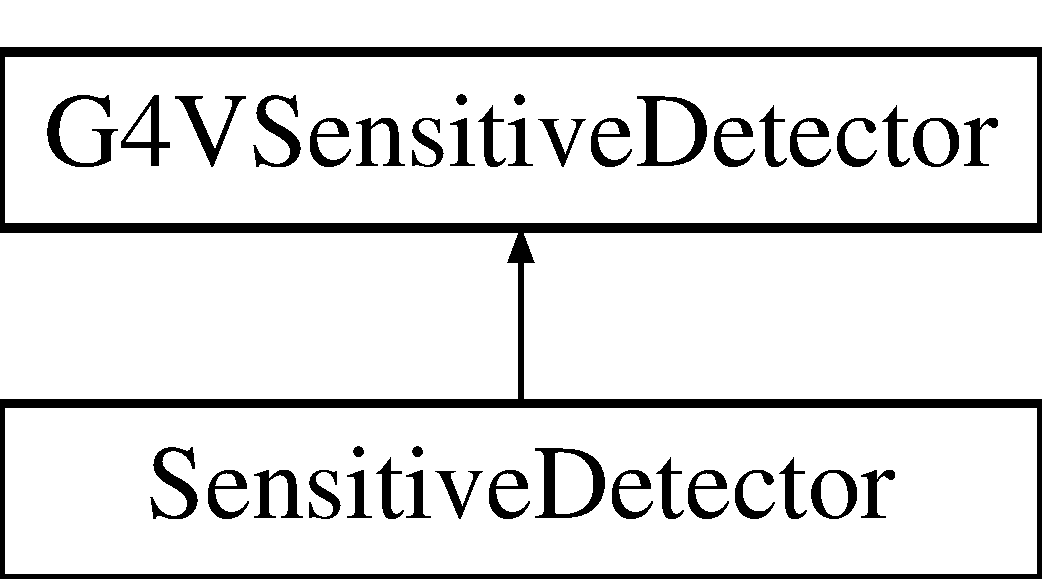
\includegraphics[height=2.000000cm]{class_sensitive_detector}
\end{center}
\end{figure}
\subsection*{Public Member Functions}
\begin{DoxyCompactItemize}
\item 
\hypertarget{class_sensitive_detector_ac88a17313a09d79b33525ebd71d0bcfd}{}\label{class_sensitive_detector_ac88a17313a09d79b33525ebd71d0bcfd} 
{\bfseries Sensitive\+Detector} (const G4\+String \&name, const G4\+String \&hits\+Collection\+Name)
\item 
\hypertarget{class_sensitive_detector_ac8d4fb05e49fbd3d7036723cf7c6afe4}{}\label{class_sensitive_detector_ac8d4fb05e49fbd3d7036723cf7c6afe4} 
virtual void {\bfseries Initialize} (G4\+H\+Cof\+This\+Event $\ast$hit\+Collection)
\item 
\hypertarget{class_sensitive_detector_a0d76f2cb50f6b3736e80d0aa99ad8ccd}{}\label{class_sensitive_detector_a0d76f2cb50f6b3736e80d0aa99ad8ccd} 
virtual G4bool {\bfseries Process\+Hits} (G4\+Step $\ast$step, G4\+Touchable\+History $\ast$history)
\item 
\hypertarget{class_sensitive_detector_a158761c11c808dc5e3724f28893e7df1}{}\label{class_sensitive_detector_a158761c11c808dc5e3724f28893e7df1} 
virtual void {\bfseries End\+Of\+Event} (G4\+H\+Cof\+This\+Event $\ast$hit\+Collection)
\end{DoxyCompactItemize}


The documentation for this class was generated from the following files\+:\begin{DoxyCompactItemize}
\item 
/\+Users/\+Hellfeld/\+Documents/\+School/\+U\+C\+B/\+Research/\+P\+R\+I\+S\+M/\+Simulations/\+P\+R\+I\+S\+M\+\_\+\+Sim/\+P\+R\+I\+S\+M\+\_\+\+Sim/include/Sensitive\+Detector.\+hh\item 
/\+Users/\+Hellfeld/\+Documents/\+School/\+U\+C\+B/\+Research/\+P\+R\+I\+S\+M/\+Simulations/\+P\+R\+I\+S\+M\+\_\+\+Sim/\+P\+R\+I\+S\+M\+\_\+\+Sim/src/Sensitive\+Detector.\+cc\end{DoxyCompactItemize}

\hypertarget{class_source_info}{}\section{Source\+Info Class Reference}
\label{class_source_info}\index{Source\+Info@{Source\+Info}}
\subsection*{Public Member Functions}
\begin{DoxyCompactItemize}
\item 
\hypertarget{class_source_info_a4f4c79089d3b673c983b3386af781252}{}\label{class_source_info_a4f4c79089d3b673c983b3386af781252} 
void {\bfseries Set\+Dir} (G4\+Three\+Vector dir\+\_\+)
\item 
\hypertarget{class_source_info_a74b66677c80b7faf1fdbe24c30e5ba47}{}\label{class_source_info_a74b66677c80b7faf1fdbe24c30e5ba47} 
void {\bfseries Set\+Pos} (G4\+Three\+Vector pos\+\_\+)
\item 
\hypertarget{class_source_info_a4cba34710c2597da406874c2f27e5a36}{}\label{class_source_info_a4cba34710c2597da406874c2f27e5a36} 
G4\+Three\+Vector {\bfseries Get\+Dir} ()
\item 
\hypertarget{class_source_info_a1faaa44f3f69a0c251cf3339f8332092}{}\label{class_source_info_a1faaa44f3f69a0c251cf3339f8332092} 
G4\+Three\+Vector {\bfseries Get\+Pos} ()
\end{DoxyCompactItemize}


The documentation for this class was generated from the following file\+:\begin{DoxyCompactItemize}
\item 
/\+Users/\+Hellfeld/\+Documents/\+School/\+U\+C\+B/\+Research/\+P\+R\+I\+S\+M/\+Simulations/\+P\+R\+I\+S\+M\+\_\+\+Sim/\+P\+R\+I\+S\+M\+\_\+\+Sim/include/Primary\+Generator\+Action.\+hh\end{DoxyCompactItemize}

\hypertarget{class_stacking_action}{}\section{Stacking\+Action Class Reference}
\label{class_stacking_action}\index{Stacking\+Action@{Stacking\+Action}}
Inheritance diagram for Stacking\+Action\+:\begin{figure}[H]
\begin{center}
\leavevmode
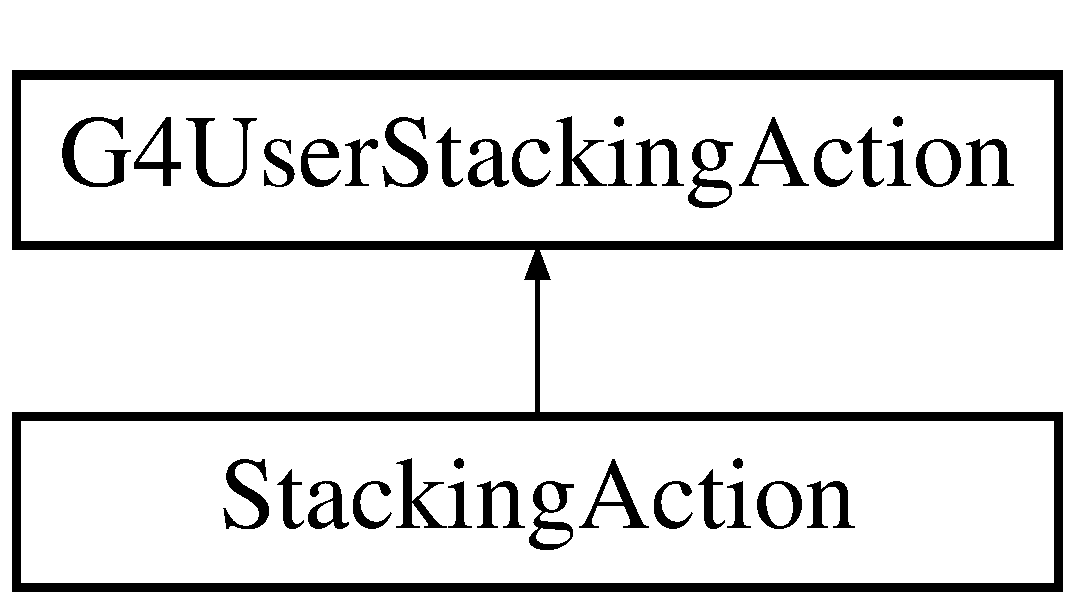
\includegraphics[height=2.000000cm]{class_stacking_action}
\end{center}
\end{figure}
\subsection*{Public Member Functions}
\begin{DoxyCompactItemize}
\item 
\hypertarget{class_stacking_action_af4780653d9e224f8d75d60e47005ea9b}{}\label{class_stacking_action_af4780653d9e224f8d75d60e47005ea9b} 
virtual G4\+Classification\+Of\+New\+Track {\bfseries Classify\+New\+Track} (const G4\+Track $\ast$)
\item 
\hypertarget{class_stacking_action_a2ac15000ac08f0f58278316e0225476b}{}\label{class_stacking_action_a2ac15000ac08f0f58278316e0225476b} 
void {\bfseries Set\+Electron\+Tracking} (G4bool gt)
\item 
\hypertarget{class_stacking_action_a5151519faf863ff7f6be8c3cf09ef412}{}\label{class_stacking_action_a5151519faf863ff7f6be8c3cf09ef412} 
G4bool {\bfseries Get\+Electron\+Tracking} ()
\end{DoxyCompactItemize}
\subsection*{Static Public Member Functions}
\begin{DoxyCompactItemize}
\item 
\hypertarget{class_stacking_action_a79aa8eb0da18014a9c1a982f3b4adf65}{}\label{class_stacking_action_a79aa8eb0da18014a9c1a982f3b4adf65} 
static \hyperlink{class_stacking_action}{Stacking\+Action} $\ast$ {\bfseries Instance} ()
\end{DoxyCompactItemize}
\subsection*{Public Attributes}
\begin{DoxyCompactItemize}
\item 
\hypertarget{class_stacking_action_a5726770e0936fcae982b2576c7391135}{}\label{class_stacking_action_a5726770e0936fcae982b2576c7391135} 
G4bool {\bfseries electrontracking}
\item 
\hypertarget{class_stacking_action_afe6d3b915ea88fd4a19b9776155600a7}{}\label{class_stacking_action_afe6d3b915ea88fd4a19b9776155600a7} 
\hyperlink{class_stacking_action_messenger}{Stacking\+Action\+Messenger} $\ast$ {\bfseries stackingactionmessenger}
\end{DoxyCompactItemize}


The documentation for this class was generated from the following files\+:\begin{DoxyCompactItemize}
\item 
/\+Users/\+Hellfeld/\+Documents/\+School/\+U\+C\+B/\+Research/\+P\+R\+I\+S\+M/\+Simulations/\+P\+R\+I\+S\+M\+\_\+\+Sim/\+P\+R\+I\+S\+M\+\_\+\+Sim/include/Stacking\+Action.\+hh\item 
/\+Users/\+Hellfeld/\+Documents/\+School/\+U\+C\+B/\+Research/\+P\+R\+I\+S\+M/\+Simulations/\+P\+R\+I\+S\+M\+\_\+\+Sim/\+P\+R\+I\+S\+M\+\_\+\+Sim/src/Stacking\+Action.\+cc\end{DoxyCompactItemize}

\hypertarget{class_stacking_action_messenger}{}\section{Stacking\+Action\+Messenger Class Reference}
\label{class_stacking_action_messenger}\index{Stacking\+Action\+Messenger@{Stacking\+Action\+Messenger}}
Inheritance diagram for Stacking\+Action\+Messenger\+:\begin{figure}[H]
\begin{center}
\leavevmode
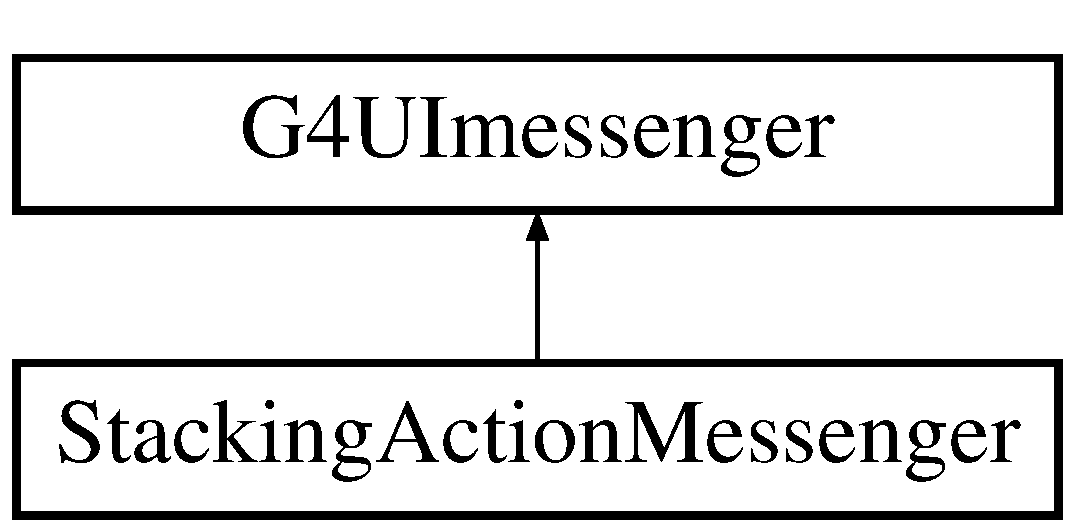
\includegraphics[height=2.000000cm]{class_stacking_action_messenger}
\end{center}
\end{figure}
\subsection*{Public Member Functions}
\begin{DoxyCompactItemize}
\item 
\hypertarget{class_stacking_action_messenger_a8c37e8a04787ecaedf44167055981ab5}{}\label{class_stacking_action_messenger_a8c37e8a04787ecaedf44167055981ab5} 
{\bfseries Stacking\+Action\+Messenger} (\hyperlink{class_stacking_action}{Stacking\+Action} $\ast$stacking)
\item 
\hypertarget{class_stacking_action_messenger_a33a2e7e11bb0f2790e6f6d25afb15842}{}\label{class_stacking_action_messenger_a33a2e7e11bb0f2790e6f6d25afb15842} 
void {\bfseries Set\+New\+Value} (G4\+U\+Icommand $\ast$command, G4\+String new\+Value)
\end{DoxyCompactItemize}


The documentation for this class was generated from the following files\+:\begin{DoxyCompactItemize}
\item 
/\+Users/\+Hellfeld/\+Documents/\+School/\+U\+C\+B/\+Research/\+P\+R\+I\+S\+M/\+Simulations/\+P\+R\+I\+S\+M\+\_\+\+Sim/\+P\+R\+I\+S\+M\+\_\+\+Sim/include/Stacking\+Action\+Messenger.\+hh\item 
/\+Users/\+Hellfeld/\+Documents/\+School/\+U\+C\+B/\+Research/\+P\+R\+I\+S\+M/\+Simulations/\+P\+R\+I\+S\+M\+\_\+\+Sim/\+P\+R\+I\+S\+M\+\_\+\+Sim/src/Stacking\+Action\+Messenger.\+cc\end{DoxyCompactItemize}

\hypertarget{class_stepping_action}{}\section{Stepping\+Action Class Reference}
\label{class_stepping_action}\index{Stepping\+Action@{Stepping\+Action}}
Inheritance diagram for Stepping\+Action\+:\begin{figure}[H]
\begin{center}
\leavevmode
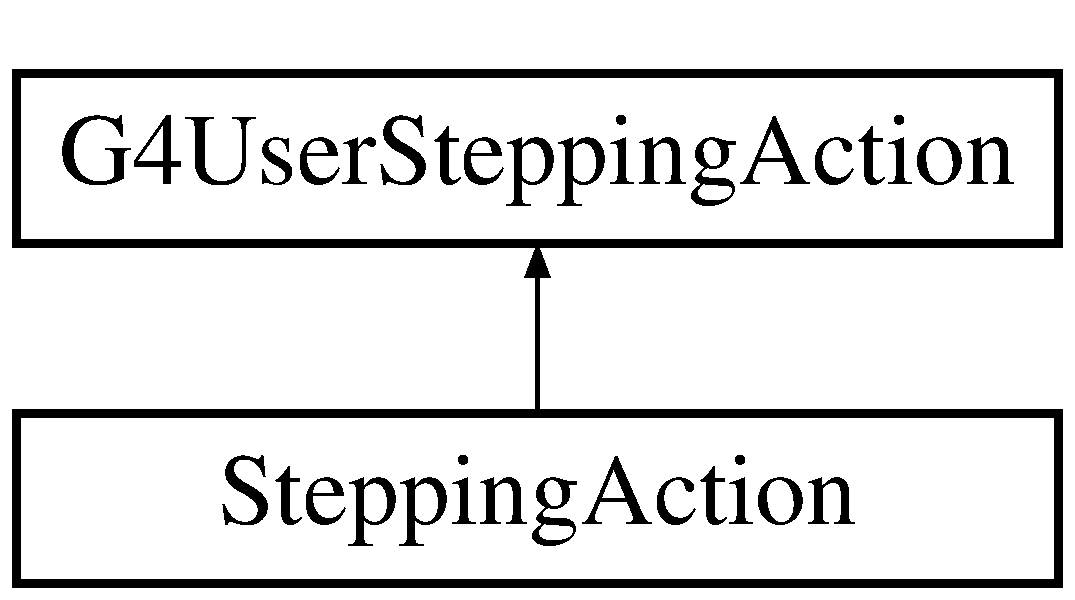
\includegraphics[height=2.000000cm]{class_stepping_action}
\end{center}
\end{figure}
\subsection*{Public Member Functions}
\begin{DoxyCompactItemize}
\item 
\hypertarget{class_stepping_action_a0b072524d0b994cff18f76270ea1ba2a}{}\label{class_stepping_action_a0b072524d0b994cff18f76270ea1ba2a} 
void {\bfseries User\+Stepping\+Action} (const G4\+Step $\ast$)
\end{DoxyCompactItemize}
\subsection*{Static Public Member Functions}
\begin{DoxyCompactItemize}
\item 
\hypertarget{class_stepping_action_af6653db032a4cf153294bfd44b13cdc5}{}\label{class_stepping_action_af6653db032a4cf153294bfd44b13cdc5} 
static \hyperlink{class_stepping_action}{Stepping\+Action} $\ast$ {\bfseries Instance} ()
\end{DoxyCompactItemize}


The documentation for this class was generated from the following files\+:\begin{DoxyCompactItemize}
\item 
/\+Users/\+Hellfeld/\+Documents/\+School/\+U\+C\+B/\+Research/\+P\+R\+I\+S\+M/\+Simulations/\+P\+R\+I\+S\+M\+\_\+\+Sim/\+P\+R\+I\+S\+M\+\_\+\+Sim/include/Stepping\+Action.\+hh\item 
/\+Users/\+Hellfeld/\+Documents/\+School/\+U\+C\+B/\+Research/\+P\+R\+I\+S\+M/\+Simulations/\+P\+R\+I\+S\+M\+\_\+\+Sim/\+P\+R\+I\+S\+M\+\_\+\+Sim/src/Stepping\+Action.\+cc\end{DoxyCompactItemize}

%--- End generated contents ---

% Index
\backmatter
\newpage
\phantomsection
\clearemptydoublepage
\addcontentsline{toc}{chapter}{Index}
\printindex

\end{document}
